\section{Results}
\label{sec:results}


\subsection{Local Fractal Dimension of Datasets}
\label{subsec:lfd-results}

Since the time complexity of CAKES algorithms scales with the local fractal dimension of the dataset, we examine the local fractal dimension of each dataset we benchmarked CAKES algorithms on.

Figure~\ref{fig:results:lfd-plots} plots LFD by depth for fashion-mnist, glove-25, sift, a random dataset, Silva 18S, and RadioML.
The horizontal axis denotes the depth in the cluster tree, and the vertical axis denotes the LFD (as calculated by Equation~\ref{eq:methods:lfd-simplified}) of clusters at that depth.
We plot lines for the 0th, 5th, 25th, 50th, 75th, 95th, and 100th percentiles of LFD.
In order to have the plots to best reflect the distribution of LFDs across the entire \emph{dataset}, we compute percentiles counting each cluster as many times as its cardinality.
In other words, if, for some dataset, the 95th percentile of LFD at depth 40 is 3, this means that 95\% of the points in clusters at depth 40 belong to a cluster whose LFD is at most 3.

Figure~\ref{fig:results:fashion-mnist-lfd} shows the LFD by depth for fashion-mnist.
We observe that until about depth 5, the LFD is low, as the 95th percentile (orange plotted line) is less than 4, and the median (red line) is just above 2.
For depths 15 through 25, we observe that the LFD increases, with the 95th percentile (orange plotted line) slightly less than 6, and the median near 3.
Finally, for depths 25 through the maximum depth, we observe that the LFD decreases again, as the 95th percentile is between 3 and 4, and the median is less than 2.

Relative to fashion-mnist, glove-25 has low LFD, as shown in Figure~\ref{fig:results:glove-25-lfd}.
Percentile lines for glove-25 are flatter and lower, indicating that the LFD is lower across the entire dataset, and that the LFD does not vary as much by depth.
The 95th percentile of LFD is less than 3 for all depths, and the median is less than 2 for all depths. 
Before depth 25, the 95th percentile hovers near 2, and from depth 20 onward, it hovers near 3.5 before dipping sharply at the maximum depths.
The median hovers near 1.5 for all depths.

Figure~\ref{fig:results:sift-lfd} shows the LFD by depth for sift.
Until about depth 5, the 95th percentile is between 2 and 6. From about depth 5 through about depth 20, the 95th percentile is greater than 6, even exceeding 8 near depth 10.
From about depth 20 onward, the 95th percentile is less than 6, and from about depth 30 onward, it is between 3 and 4.
The median reaches its peak of about 5 at around depth 15, but hovers near 2 after about depth 30.

In contrast with Figure~\ref{fig:results:sift-lfd}, Figure~\ref{fig:results:random-lfd} shows the LFD by depth for a random dataset with the same cardinality and dimensionality as sift.
We observe that the LFD starts as high as 20 (for all data) at depth 0.
As shown by the needlepoint shape of the plot, the LFD for all clusters is about the same from depth 0 through depth 5.
After depth 5, we begin to see a wider spread between the maximum and minimum LFD at each depth.
The median decreases seemingly linearly from about 20 at depth 0 to about 2 at depth 20, remaining less than 2 for all depths greater than 20.
The LFD of approximately 20 at depth 0 is what we expect for this random dataset.
To elaborate, the distribution of points in such a dataset should reflect the curse of dimensionality, or the fact that in high dimensional spaces, the minimum and maximum pairwise distances between any two points are approximately equal.
As a result, the root cluster's radius $r$, which reflects the maximum distance between the center $c$ and any other point, should not differ significantly from the distance between the center and its closest point.
A consequence of this is that with high probability, a point in the root cluster is a distance greater than half the root radius from the center; $B_X(c, \tfrac{r}{2})$ contains only $c$ while $B_X(c, r) = |X|$, where $X$ is the dataset.
Given our definition of LFD in Equation~\ref{eq:methods:lfd-simplified}, this means that the LFD of the root cluster is approximately $\log_2(\frac{|X|}{1}) = \log_2(1,000,000) \approx 20$, which is what we observe in Figure~\ref{fig:results:random-lfd}.

Silva, as shown in Figure~\ref{fig:results:silva-lfd}, exhibits consistently low LFD.
The 95th percentile is less than about 3 for all depths, hovering near 1 for depths 40 through 128.
The median reaches its peak at 2 for about depth 10 and remains close to 0 for depths 40 through 128.

Relative to the other datasets, RadioML, as displayed in Figure~\ref{fig:results:radioml-lfd}, exhibits high LFD.
Notably however, for the first approximately 15 depths, the 95th percentile and median LFD are very close to 0.
Both percentiles increase sharply after depth 20, nearly reaching 16.
LFD remains high even as depth increases, with the 95th percentile fluctuating between about 6 and 15 for depths about 20-40.
It then spikes up again to about 10 at around depth 45 before decreasing linearly to 1 at depth 60.
The median LFD follows a similar pattern of peaks and troughs, fluctuating between about 3 and 15 for depths 20-40, spiking at about depth 50 to 5, and then decreasing approximately linearly to 1 at depth 60.

\begin{figure}
    \begin{subfigure}[b]{0.47\textwidth}
    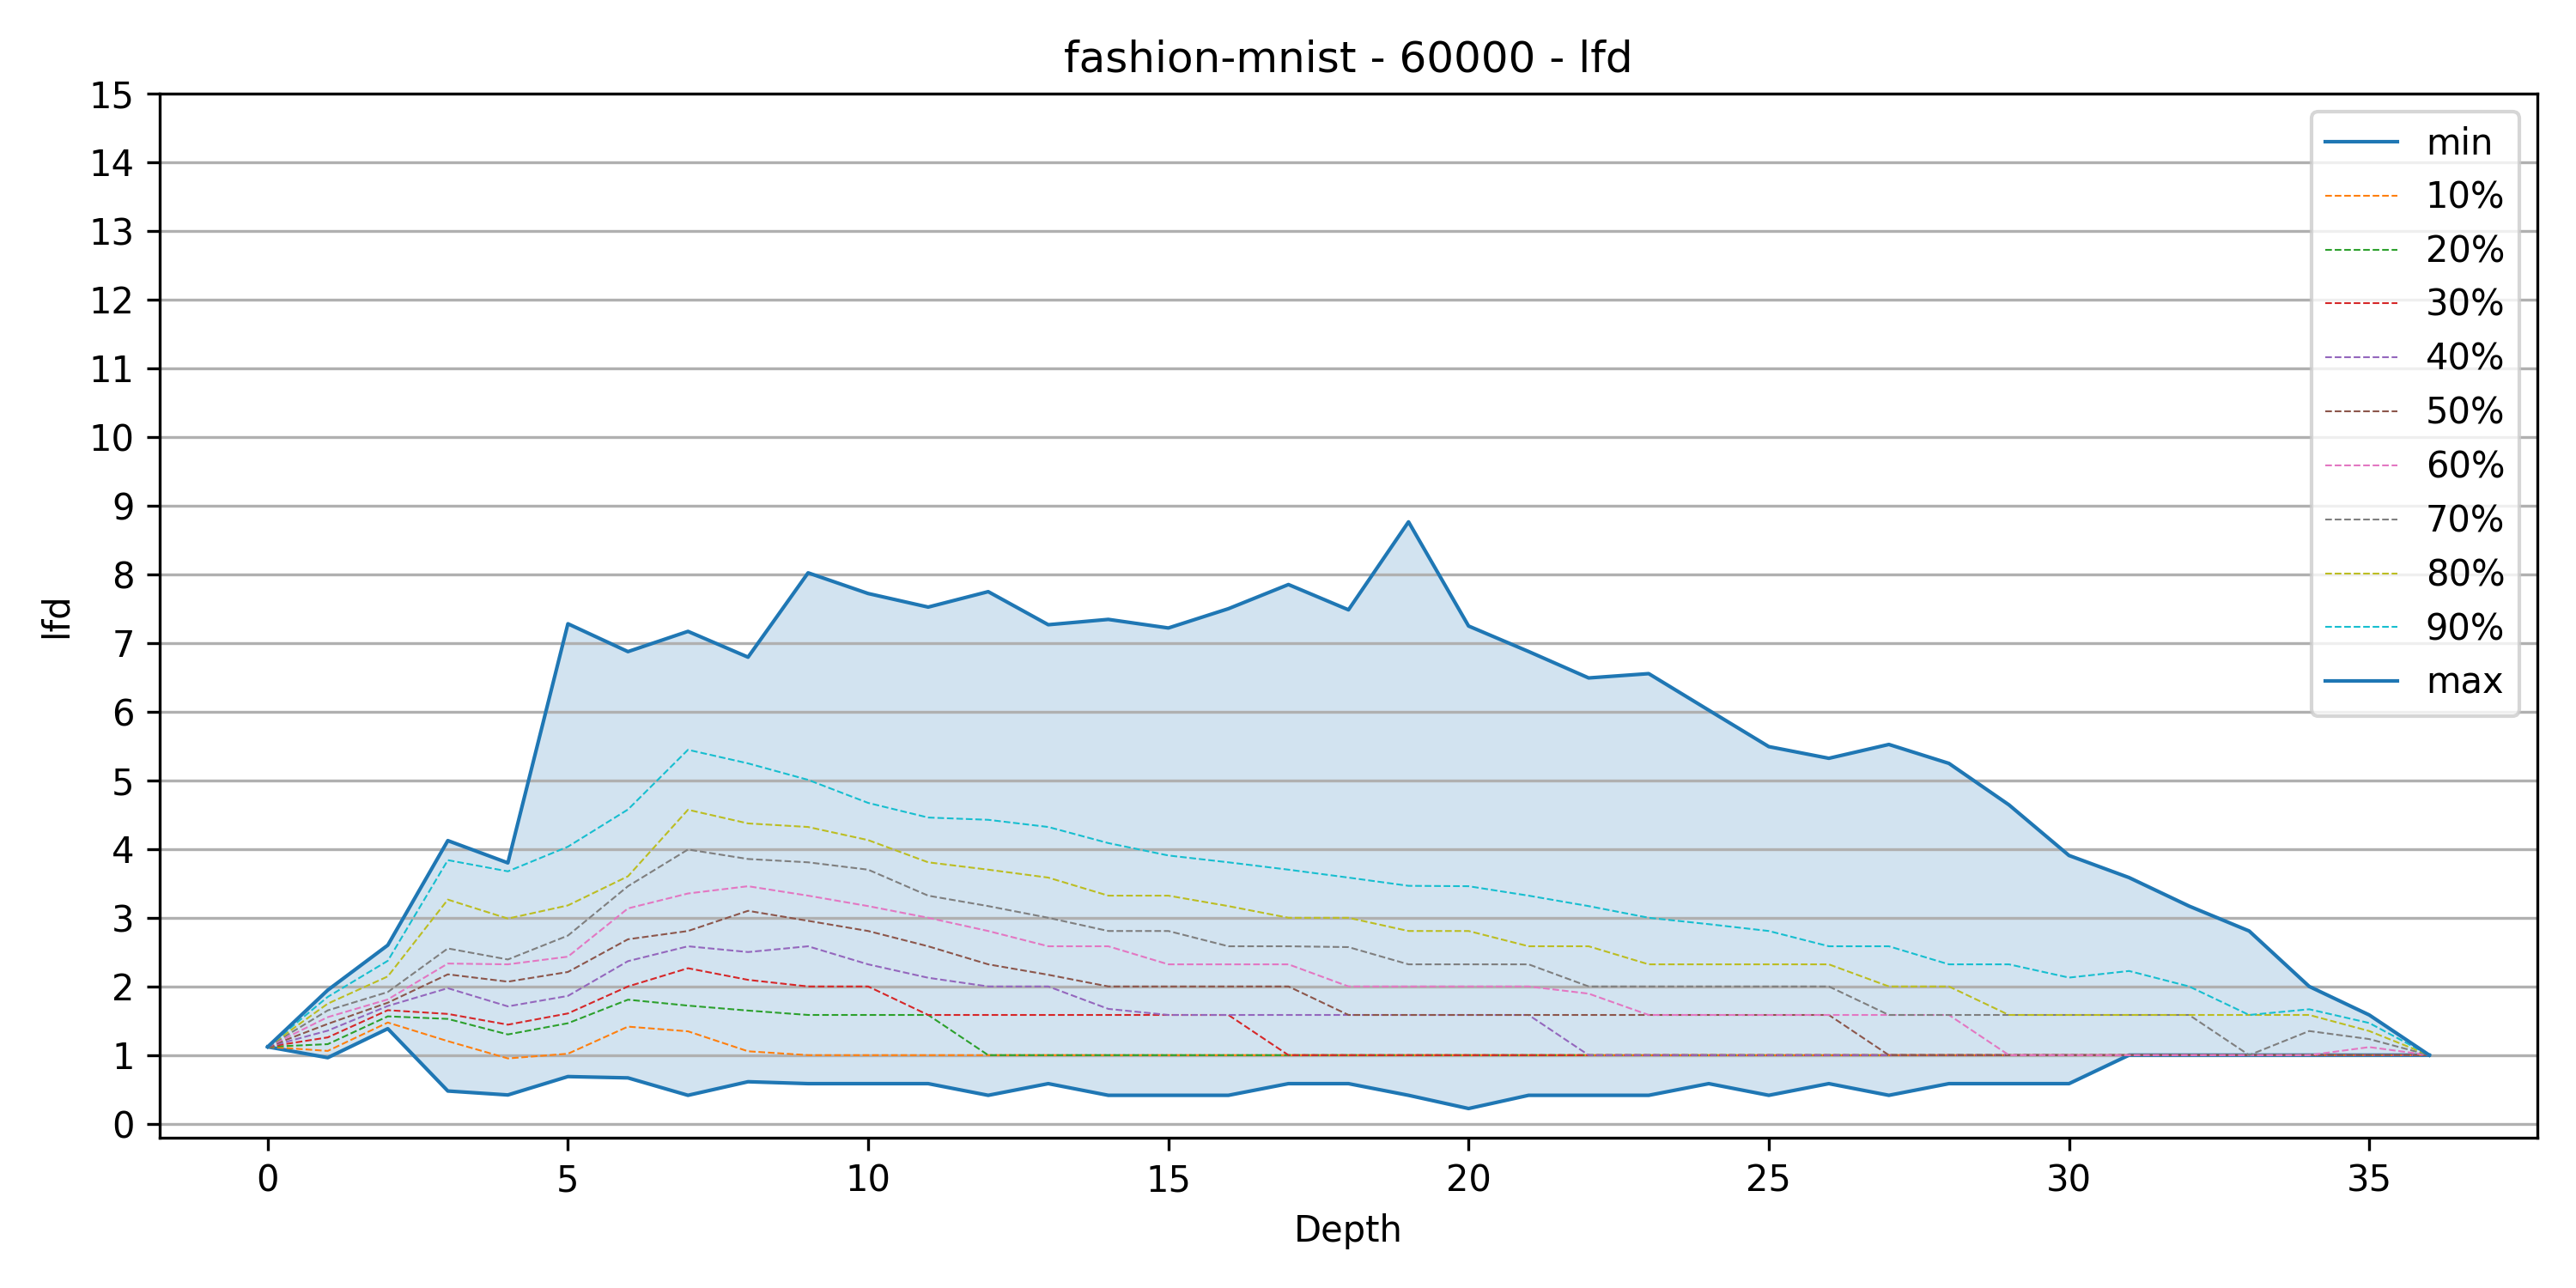
\includegraphics[width=0.95\textwidth]{images/lfd_plots/fashion-mnist-60000-lfd.png}\\
    \subcaption{Fashion-mnist}
    \label{fig:results:fashion-mnist-lfd}
    \end{subfigure}%
    \begin{subfigure}[b]{0.47\textwidth}
    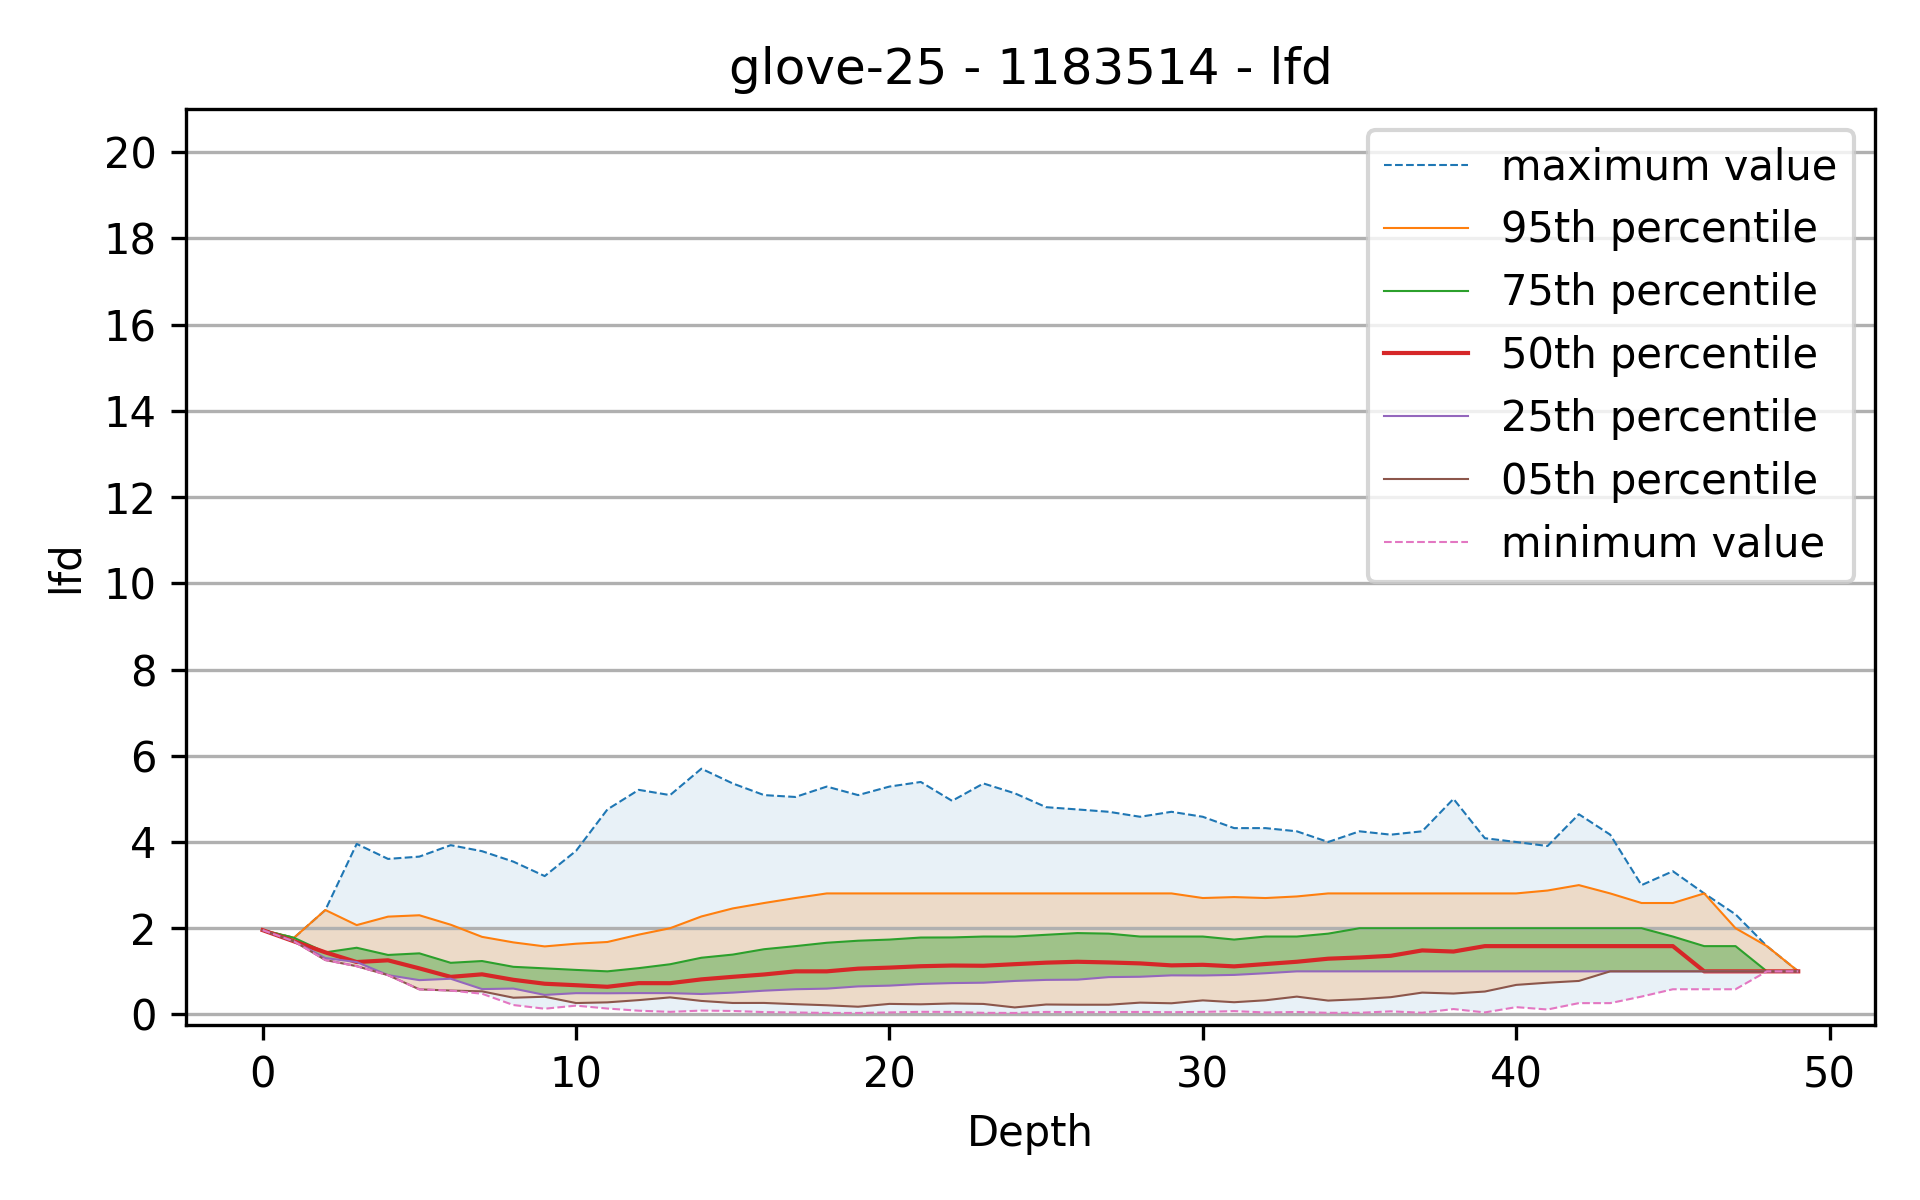
\includegraphics[width=0.95\textwidth]{images/lfd_plots/glove-25-1183514-lfd.png}\\
    \subcaption{Glove-25}
    \label{fig:results:glove-25-lfd}
    \end{subfigure}
    \vspace{1em}
    \\
    \begin{subfigure}[b]{0.47\textwidth}
    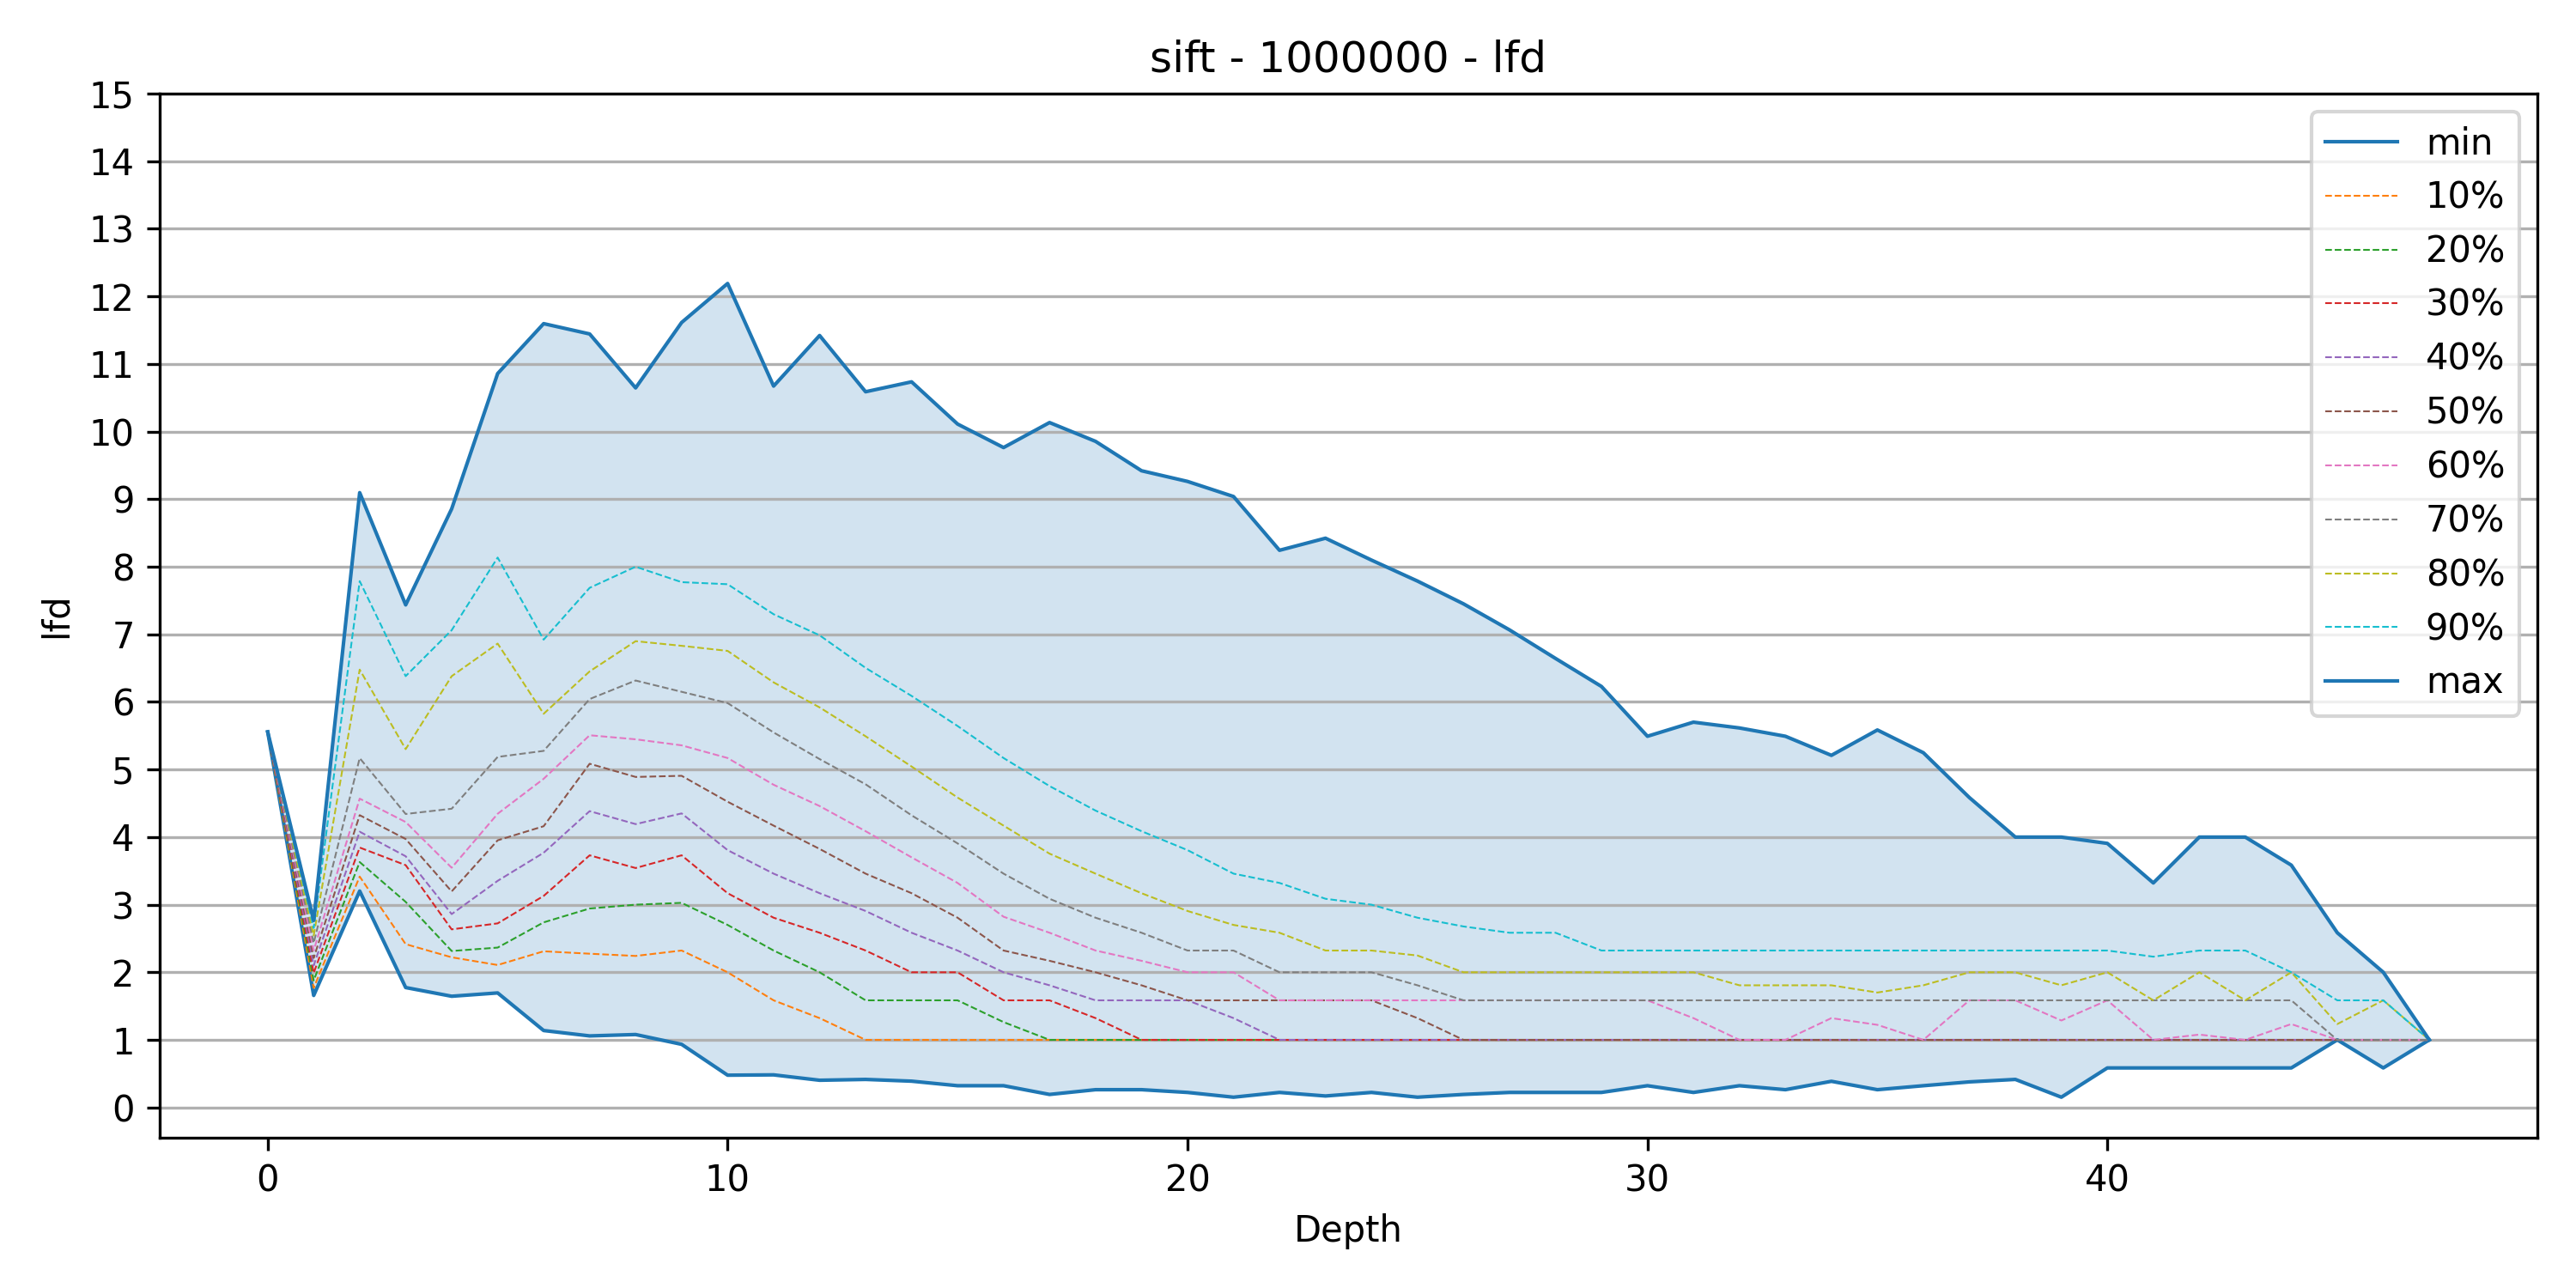
\includegraphics[width=0.95\textwidth]{images/lfd_plots/sift-1000000-lfd.png}\\
    \subcaption{Sift}
    \label{fig:results:sift-lfd}
    \end{subfigure}%
    \begin{subfigure}[b]{0.47\textwidth}
    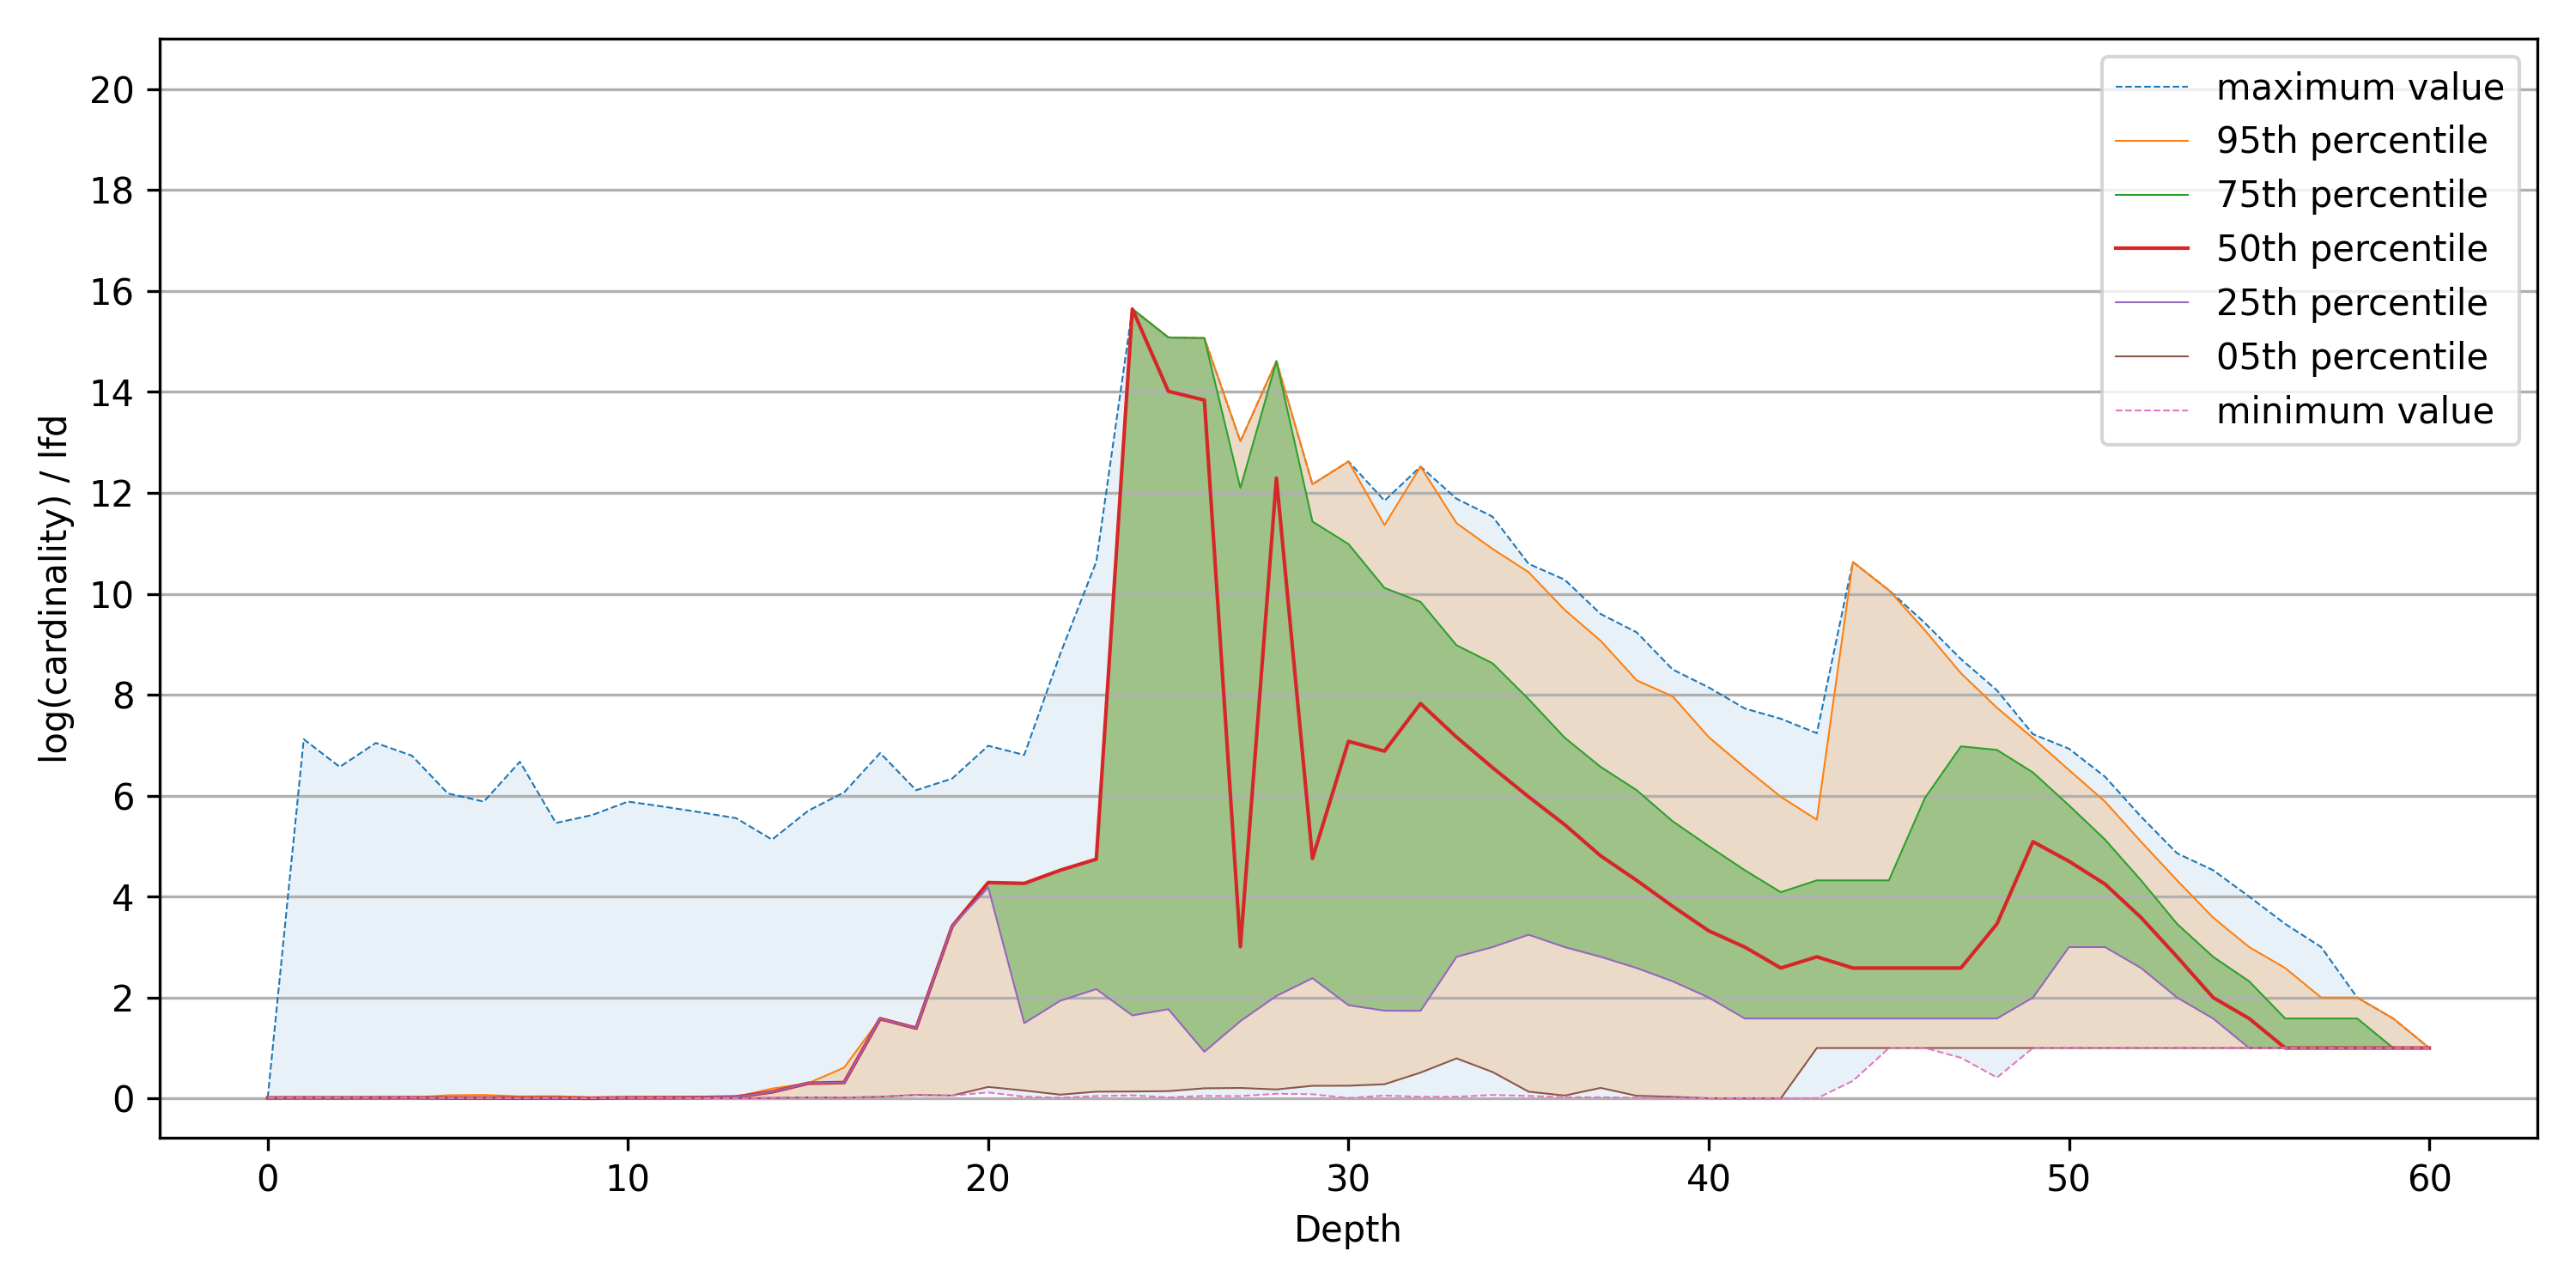
\includegraphics[width=0.95\textwidth]{images/lfd_plots/radio-ml-97920-lfd.png}\\
    \subcaption{RadioML}
    \label{fig:results:radioml-lfd}
    \end{subfigure}%
    \\
    \begin{subfigure}[b]{0.47\textwidth}
    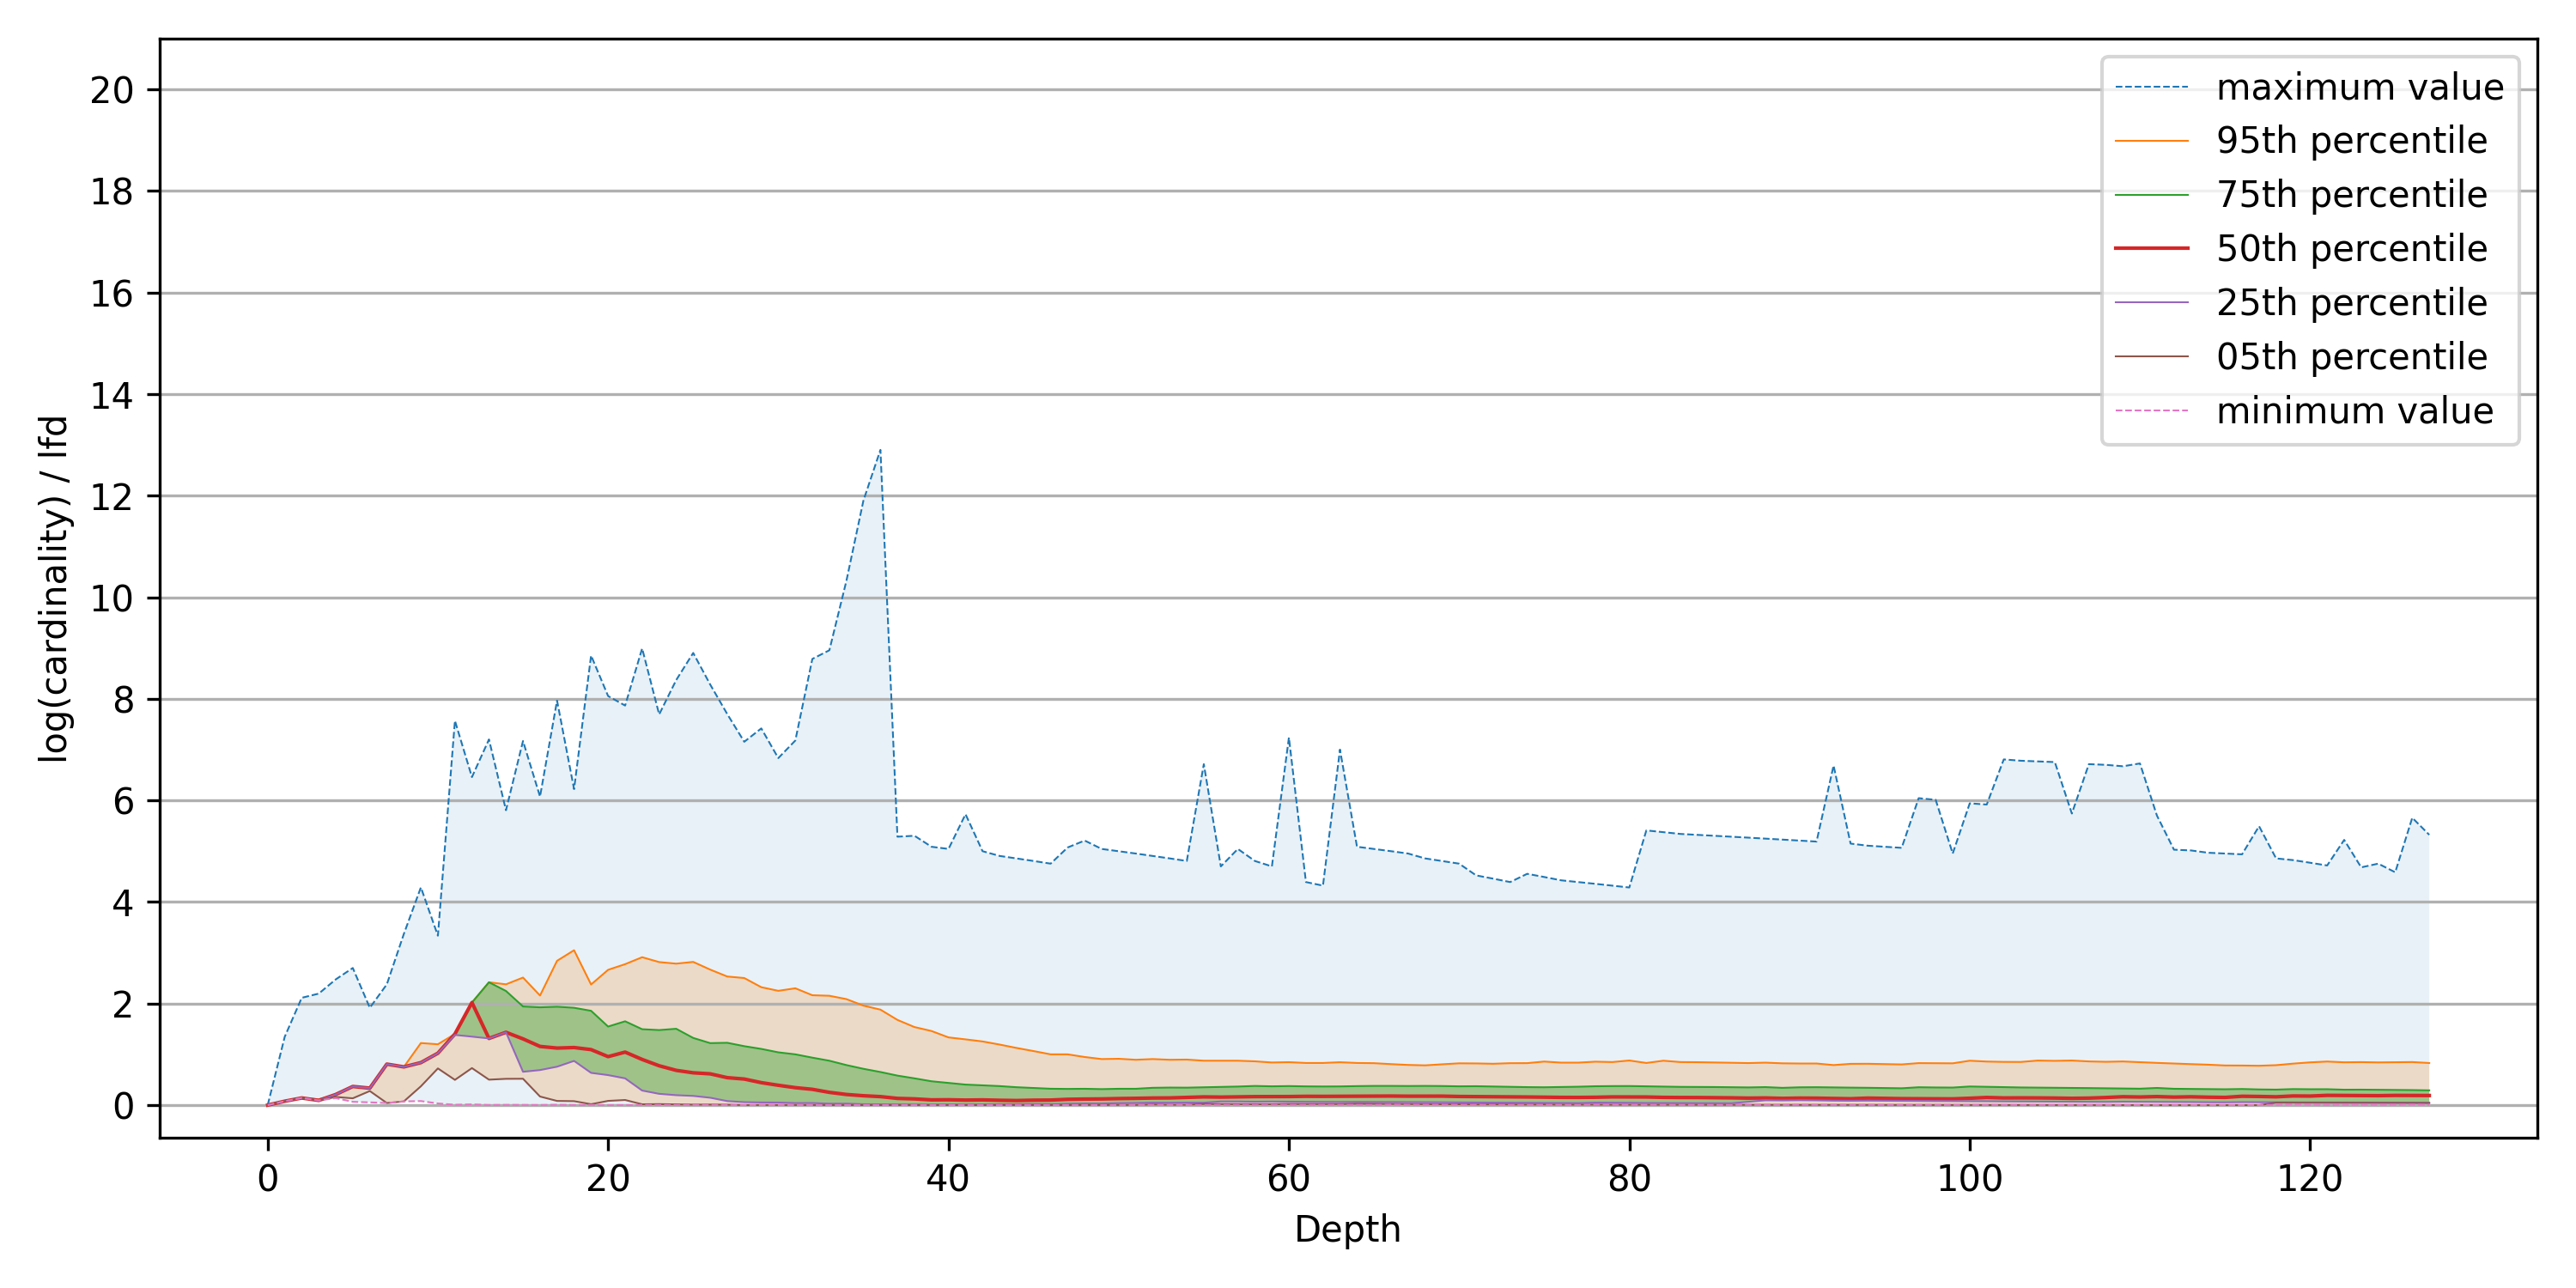
\includegraphics[width=0.95\textwidth]{images/lfd_plots/silva-2224640-lfd.png}\\
    \subcaption{Silva 18S}
    \label{fig:results:silva-lfd}
    \end{subfigure}%  
    \begin{subfigure}[b]{0.47\textwidth}
    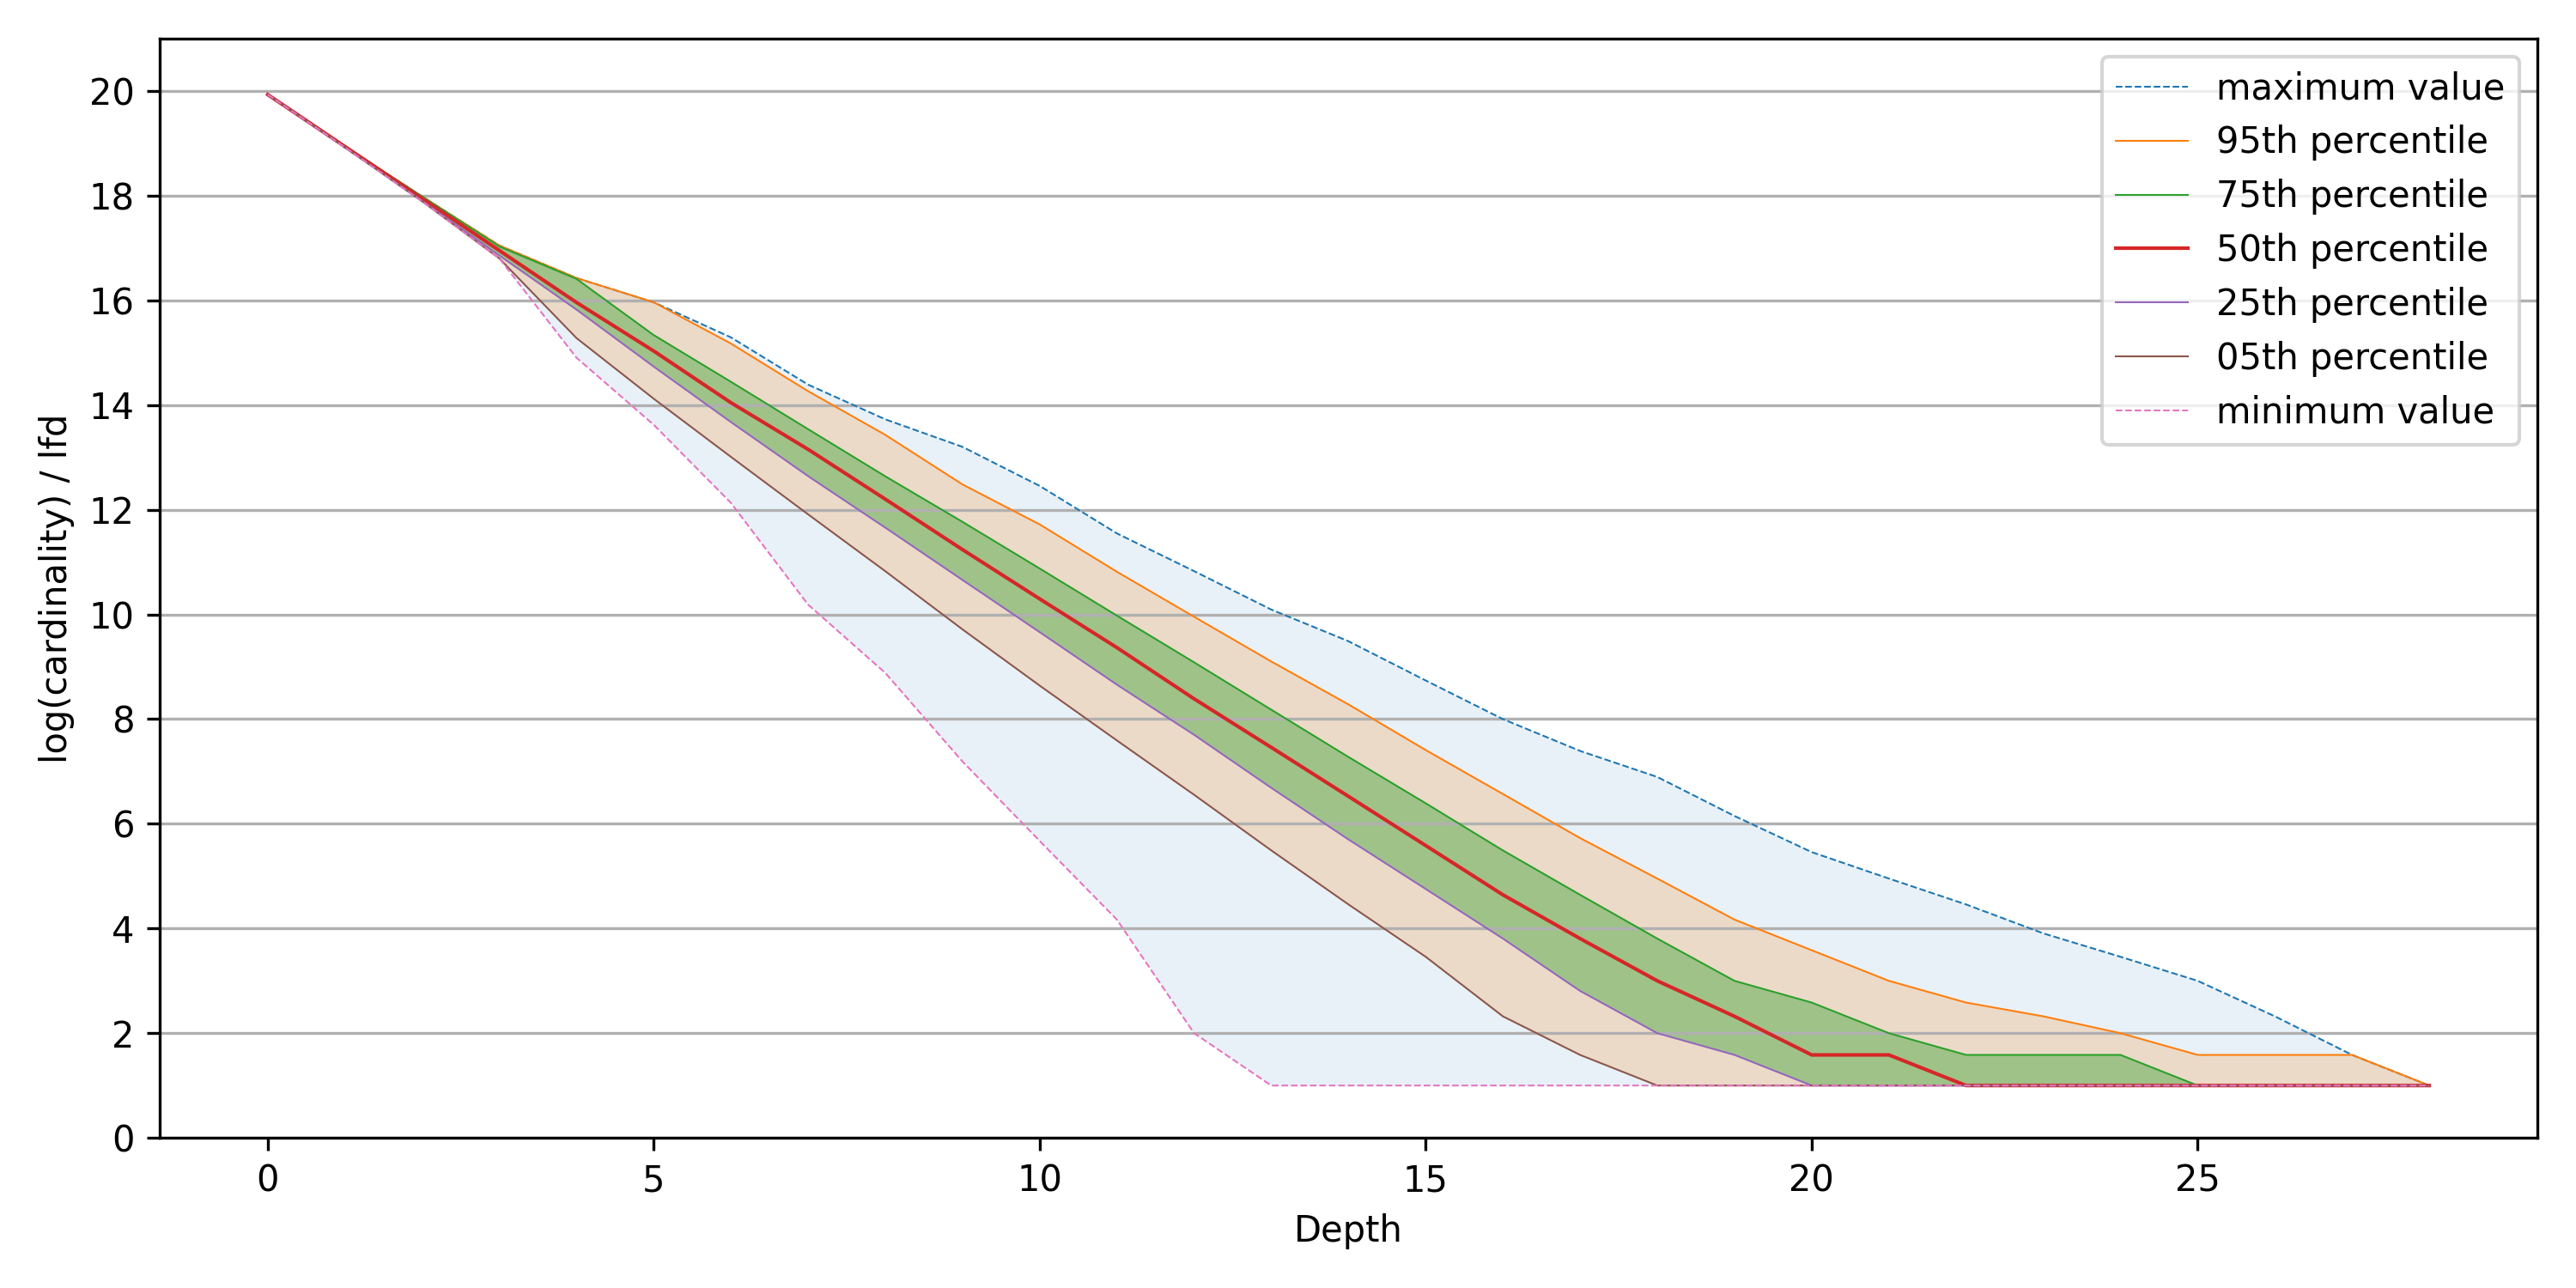
\includegraphics[width=0.95\textwidth]{images/lfd_plots/random-1000000-lfd.png}\\
    \subcaption{A random dataset}
    \label{fig:results:random-lfd}
    \end{subfigure}
    \vspace{1em}
    \caption{Local fractal dimension vs. cluster depth across six datasets, grouped by decile of local fractal dimension and weighted by the cardinalities of the clusters.
    The last dataset is randomly generated.
    {\color{red} TODO: Remove the headers from the plots themselves and rely on subcaptions instead.}}
    \label{fig:results:lfd-plots}
\end{figure}

\subsection{Indexing and Tuning Time}
\label{subsec:indexing-time-results}


For each of the ANN benchmark datasets and the Random dataset, we report the time taken for each algorithm to build the index and to tune the hyperparameters for these indices to achieve the highest possible recall (lower is better). 
Though CAKES has three different algorithms, indexing is the same for each of them, so we can simply report the indexing time for CAKES as a whole. 

The horizontal axis in each figure shows the cardinality of the augmented dataset with synthetic points (see Section \ref{subsec:methods:synthetic-data}).
The left-most point on each line is on the original dataset without any synthetic augmentation.
The vertical axis denotes throughput in queries per second.
Both axes are on a logarithmic scale.

With the Fashion-Mnist dataset, as shown in Figure~\ref{fig:results:fashion-mnist-indexing}, we observe that the indexing time for CAKES is much lower than that of HNSW, ANNOY, and FAISS-IVF, but higher than that of FAISS-Flat.
This is not surprising, given that FAISS-Flat is a naive linear search algorithm and is not building an index. 

{\color{red} TODO: Add a sentence or two about the indexing time for the other datasets.}


\begin{figure}
    \begin{subfigure}[b]{0.47\textwidth}
    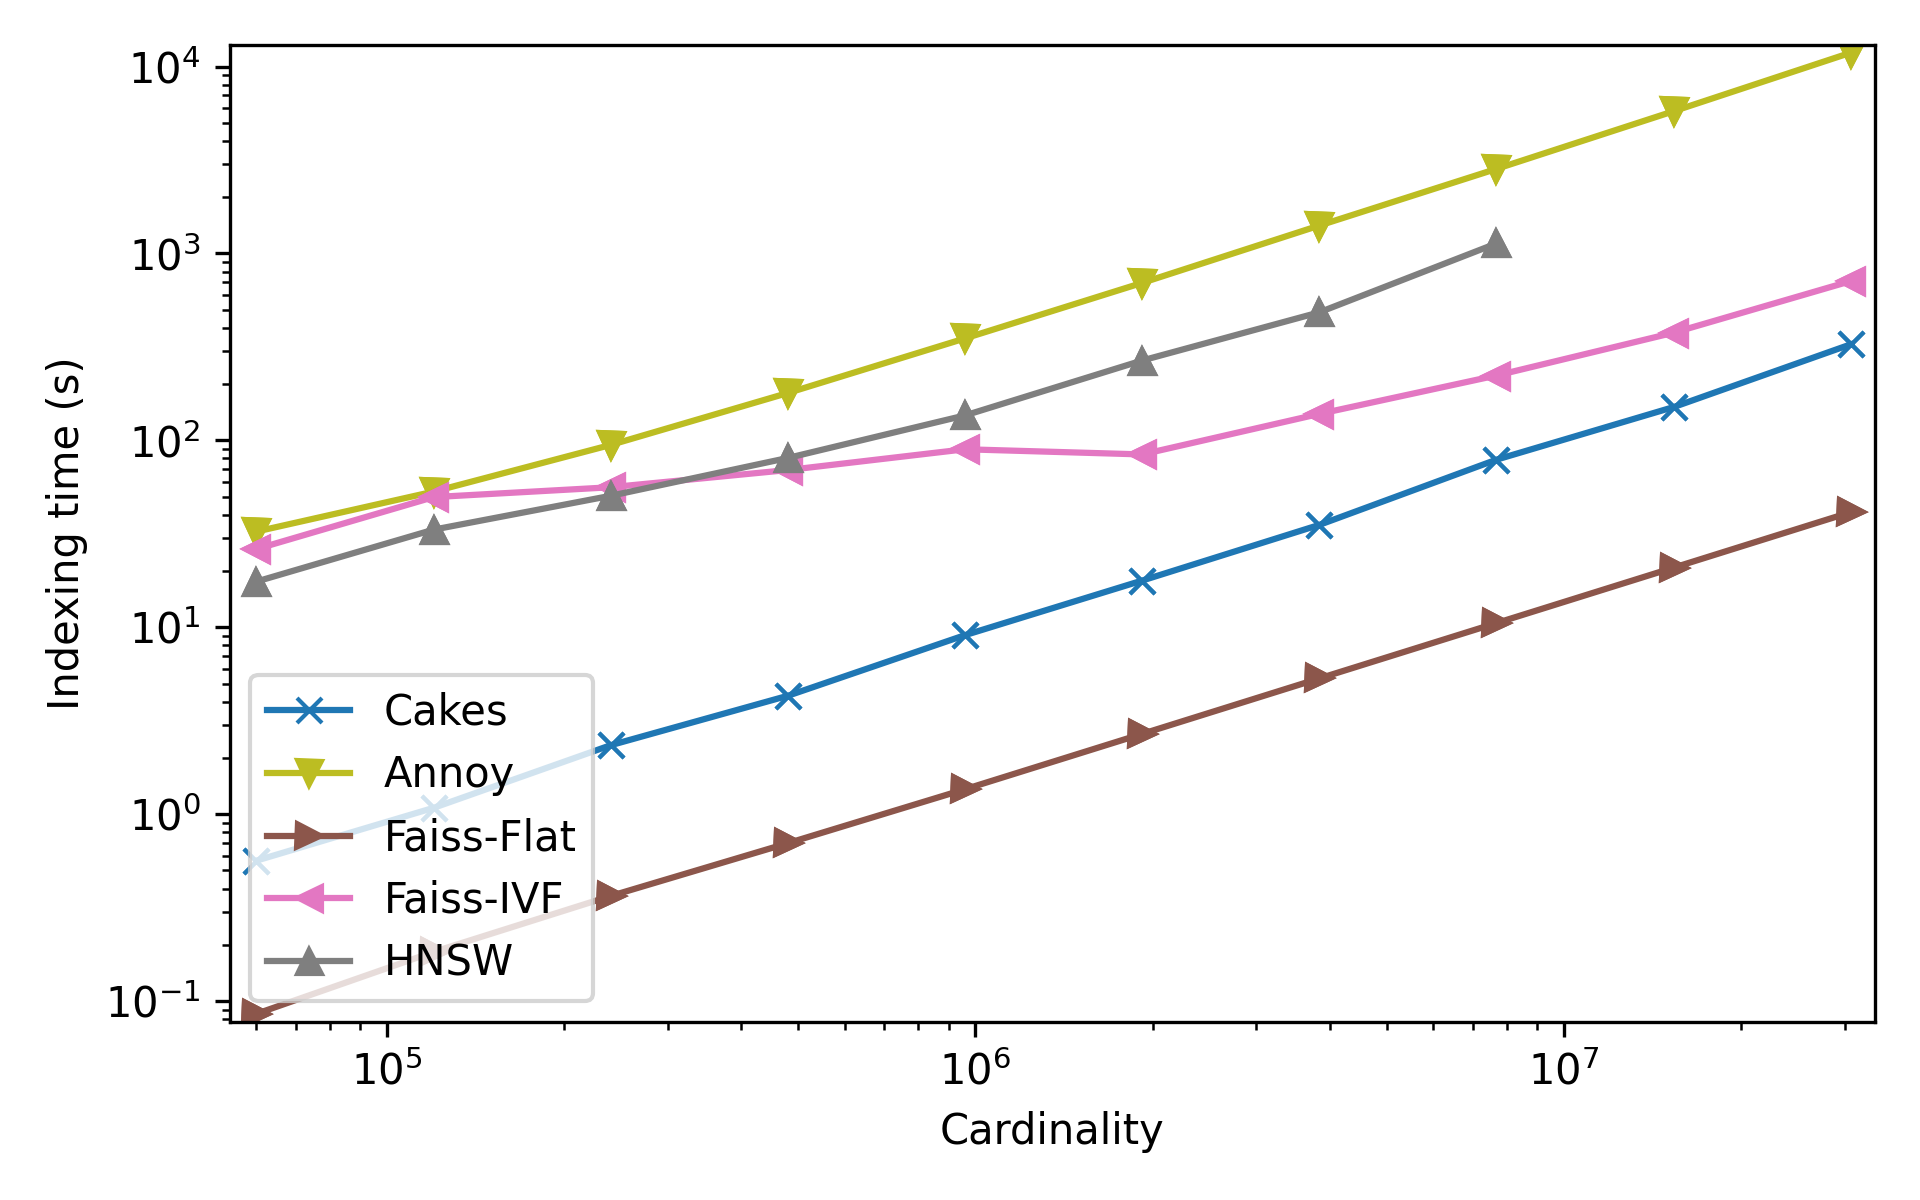
\includegraphics[width=0.95\textwidth]{plots/fashion-mnist-indexing.png}\\
    \subcaption{Fashion-mnist}
    \label{fig:results:fashion-mnist-indexing}
    \end{subfigure}%
    \begin{subfigure}[b]{0.47\textwidth}
    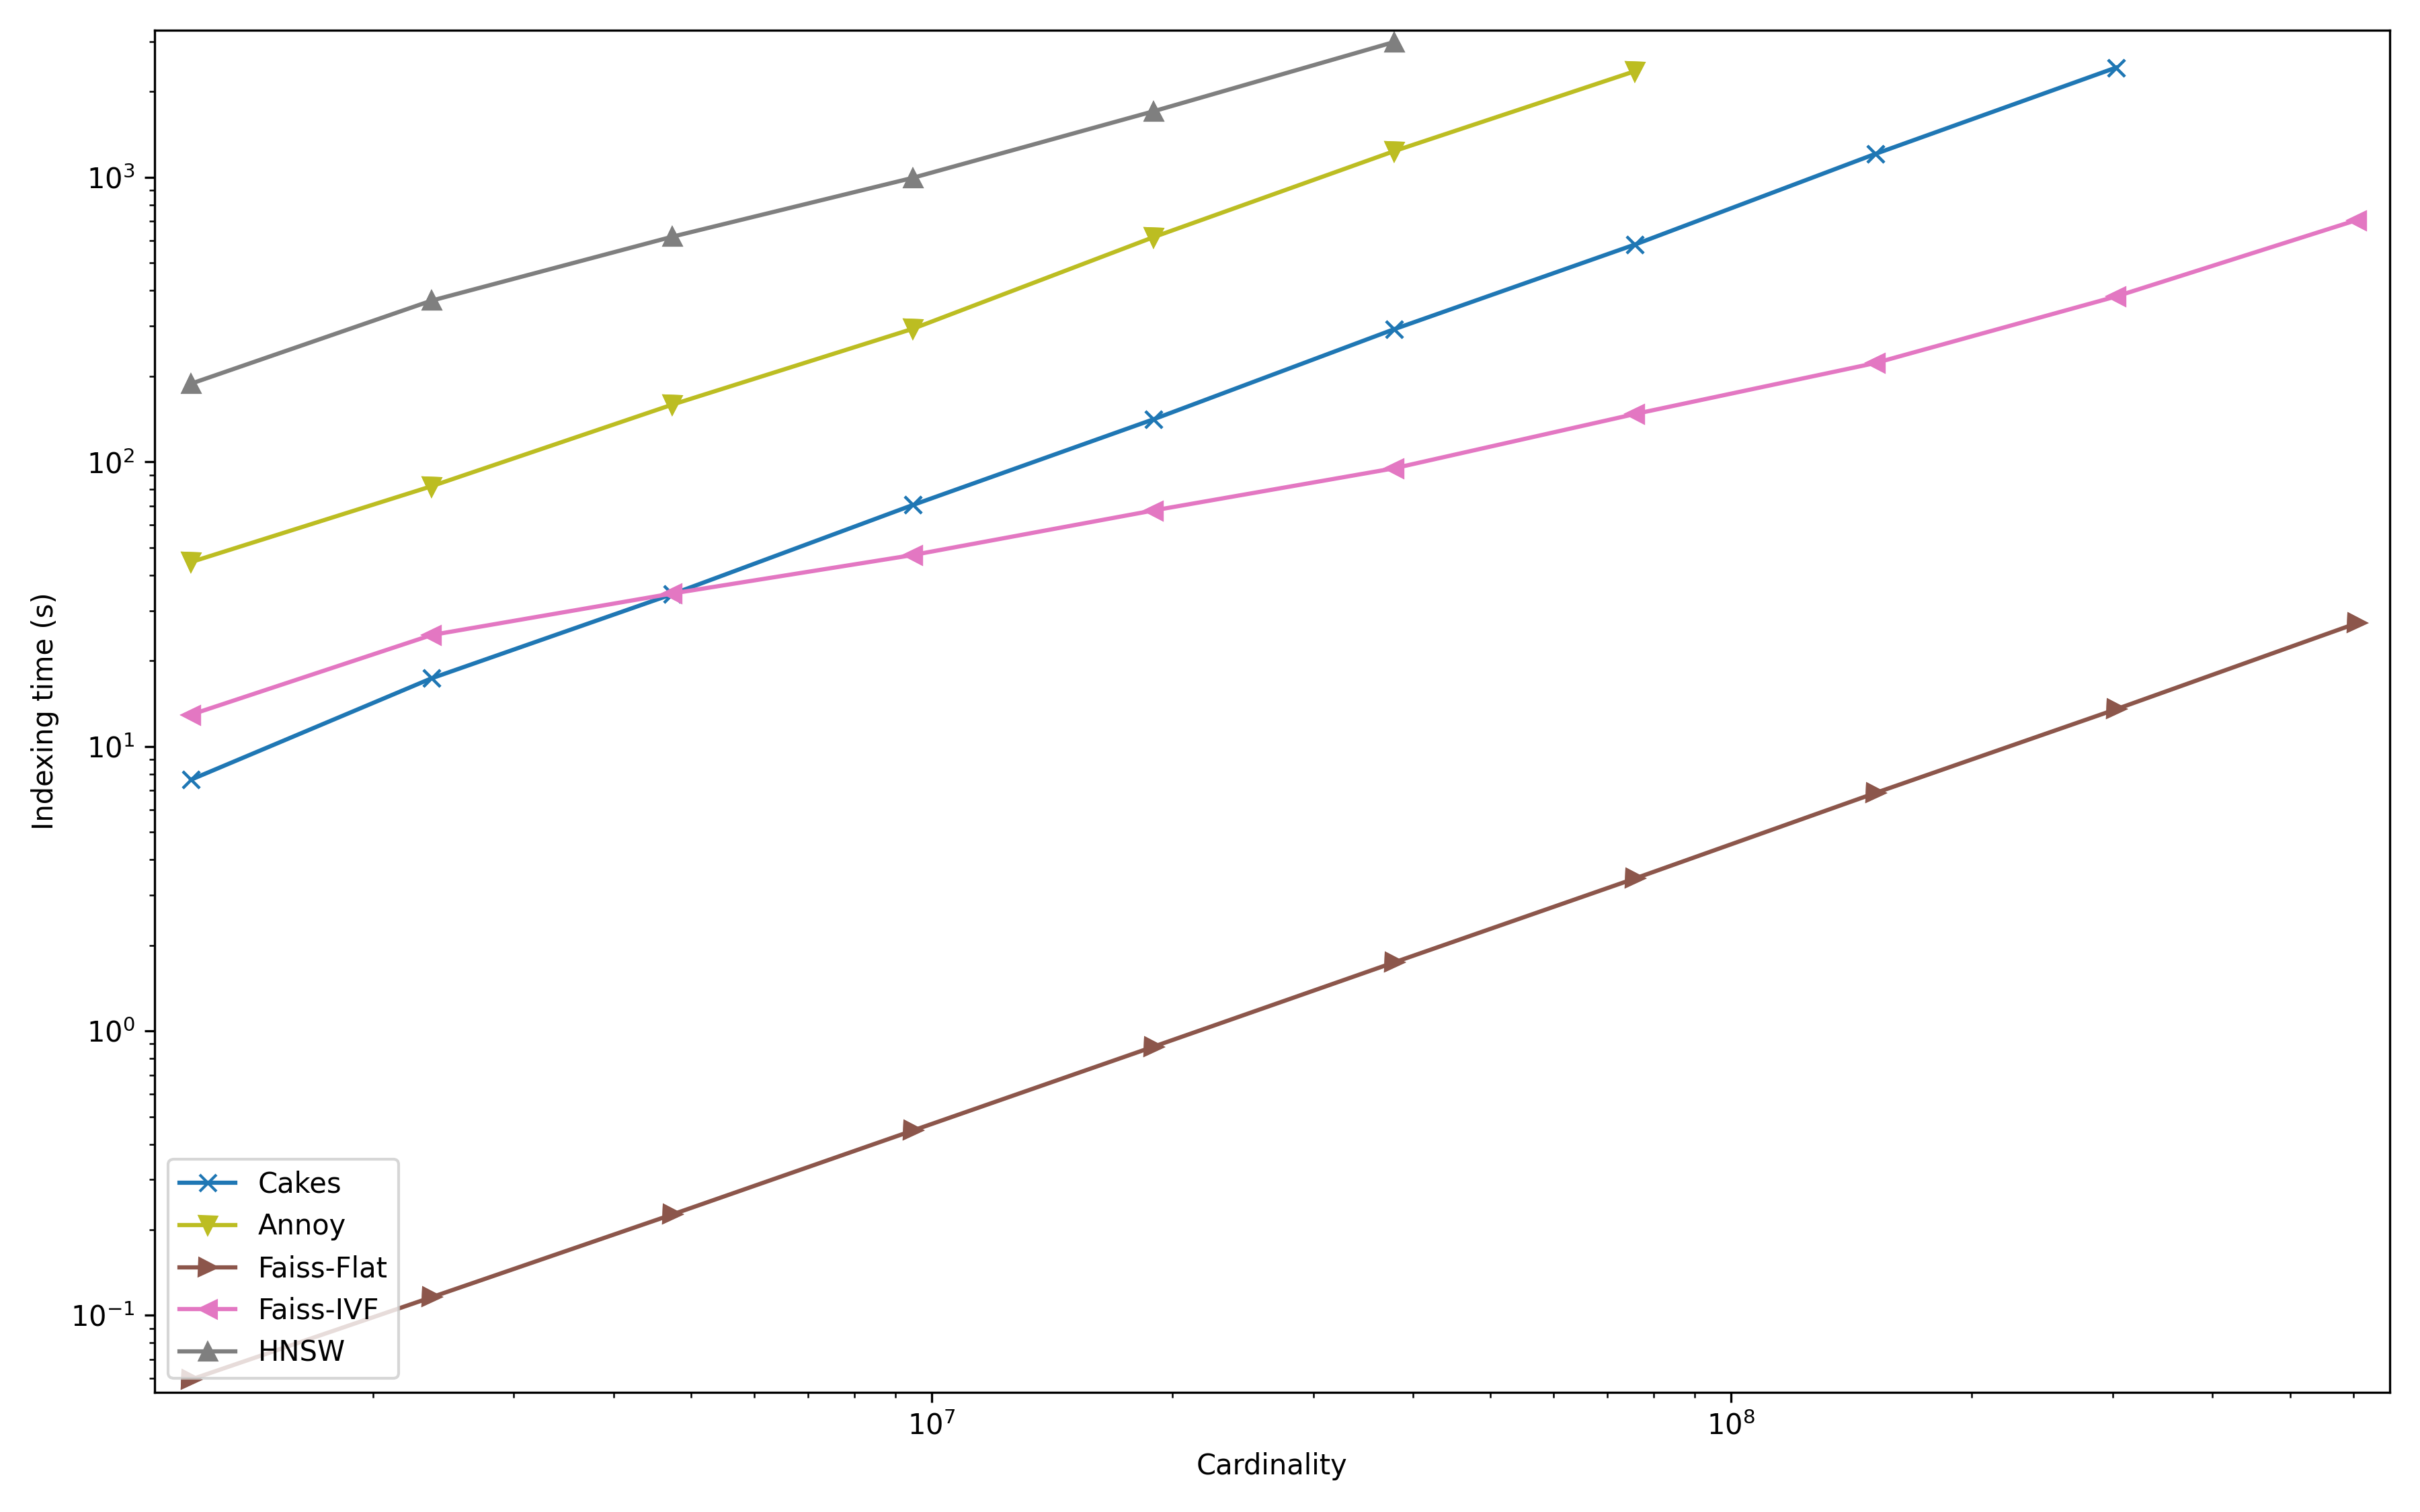
\includegraphics[width=0.95\textwidth]{plots/glove-25-indexing.png}\\
    \subcaption{Glove-25}
    \label{fig:results:glove-25-indexing}
    \end{subfigure}
    \vspace{1em}
    \\
    \begin{subfigure}[b]{0.47\textwidth}
    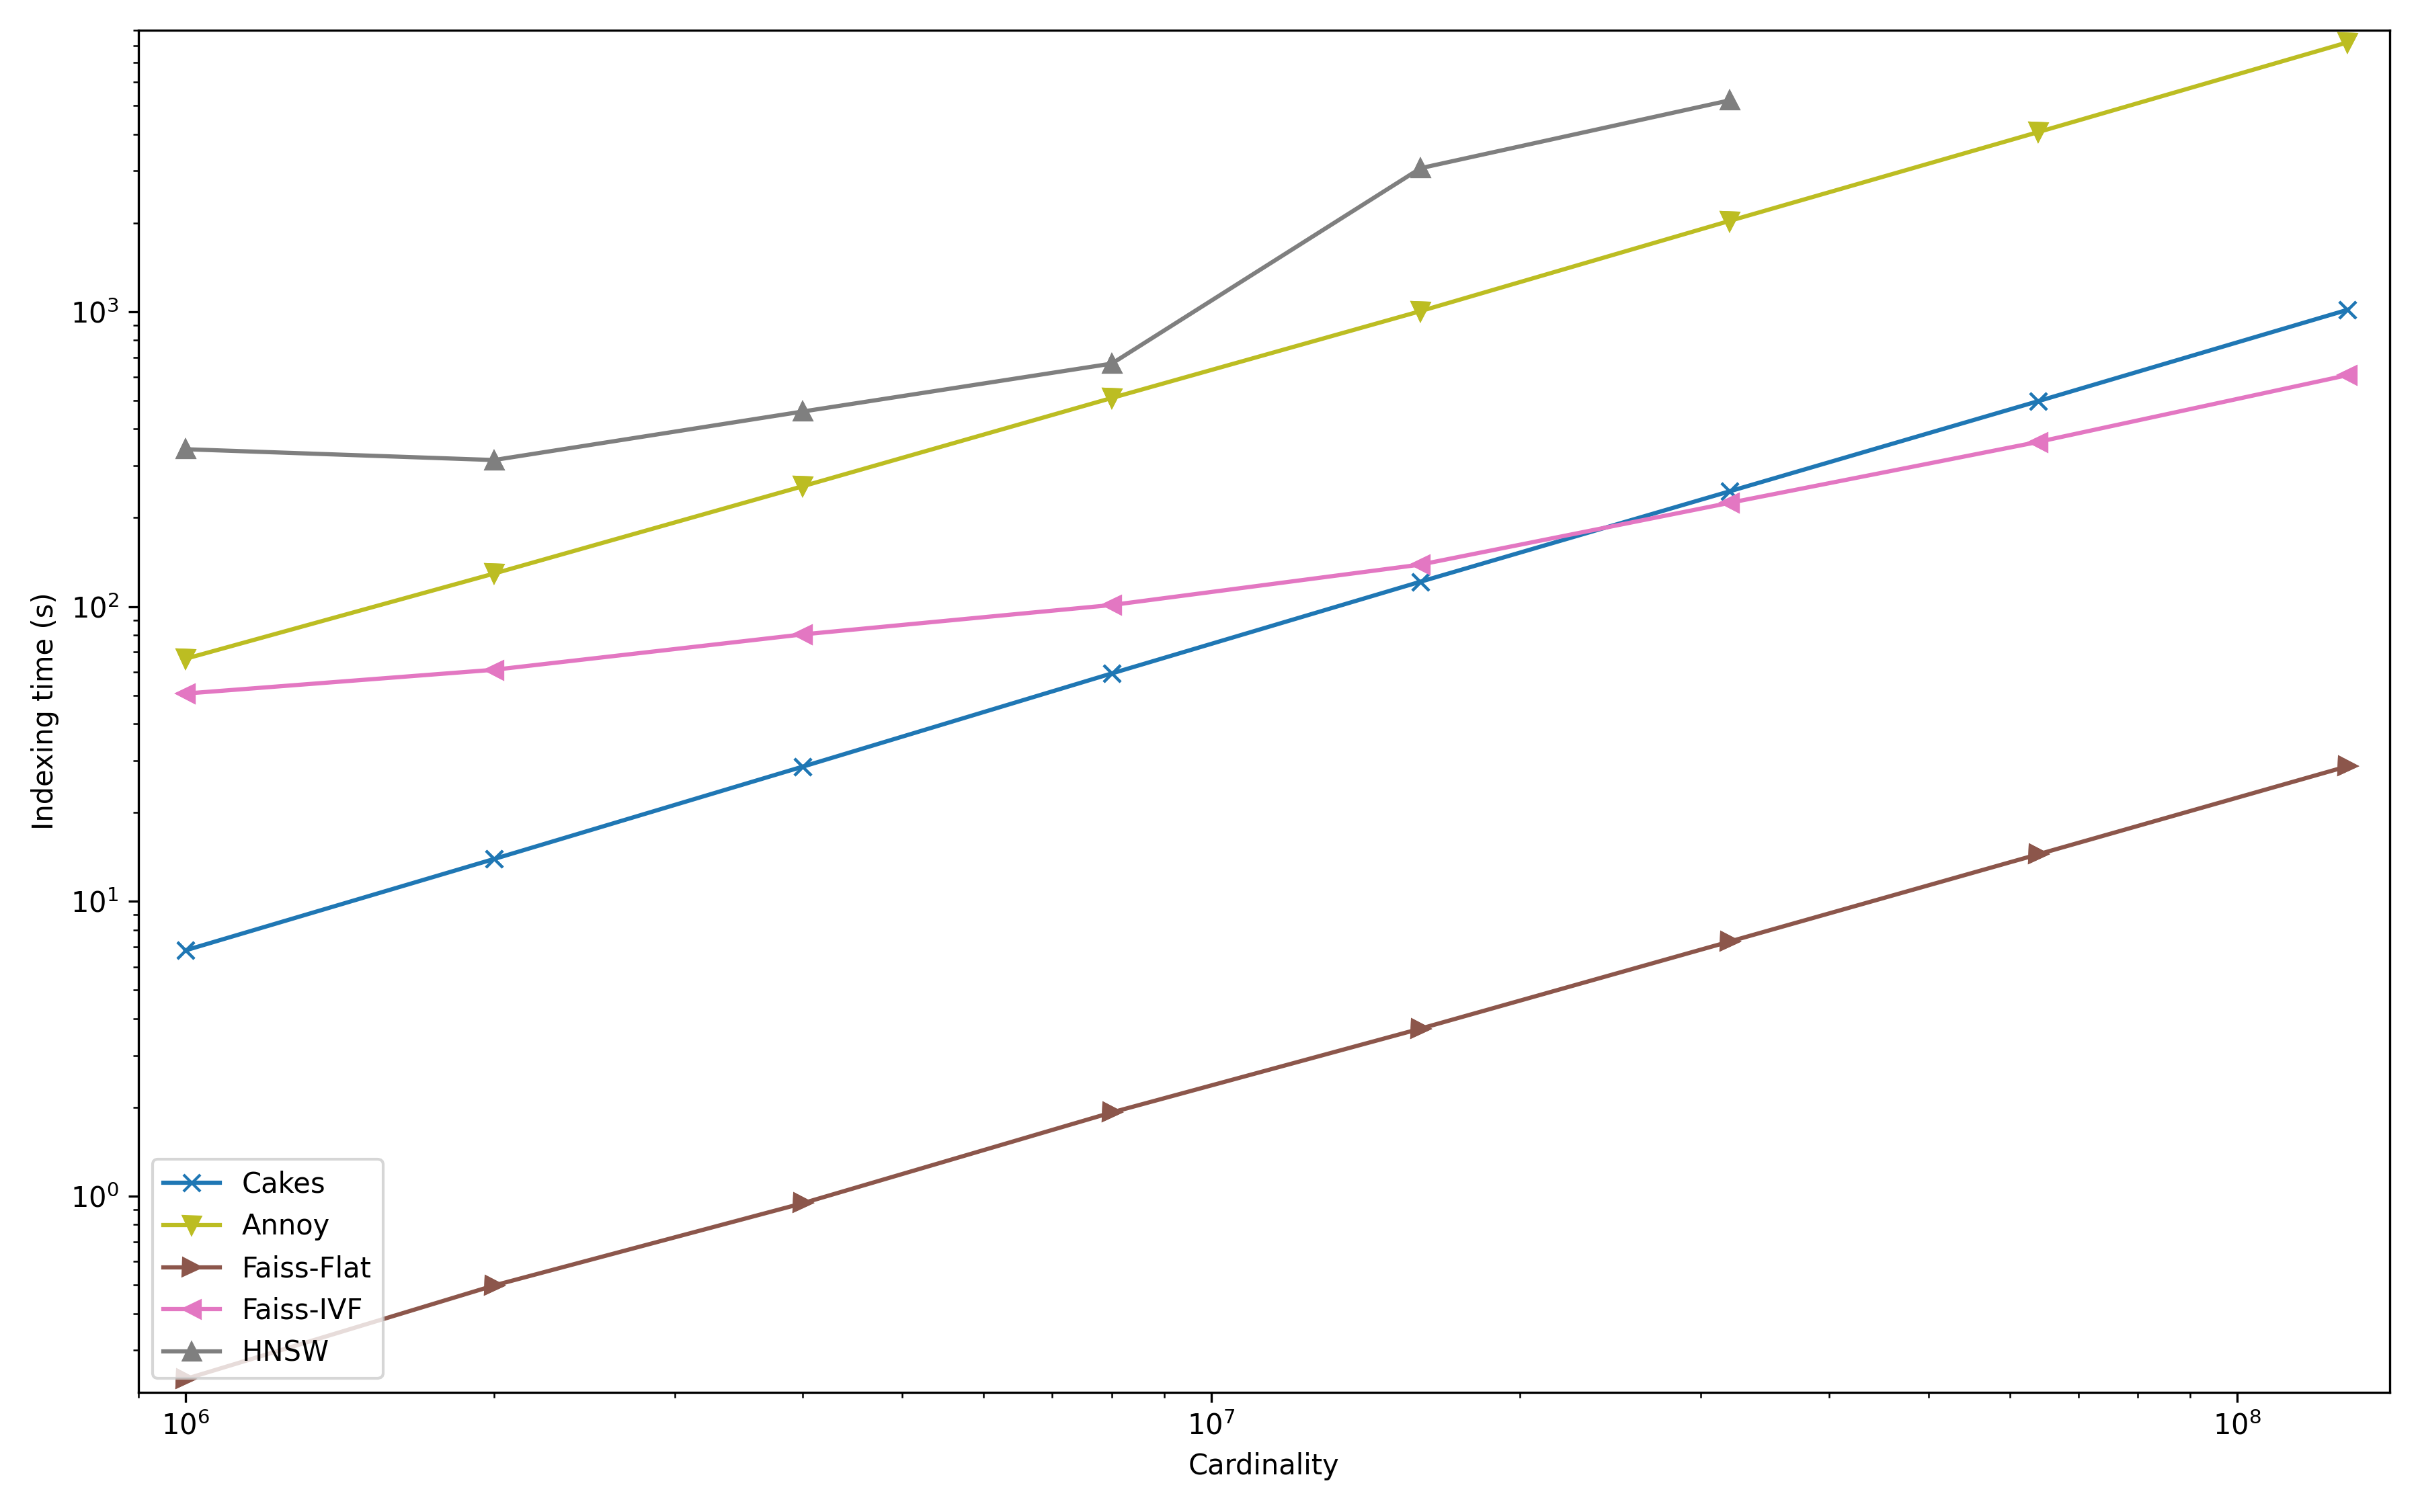
\includegraphics[width=0.95\textwidth]{plots/sift-indexing.png}\\
    \subcaption{Sift}
    \label{fig:results:sift-indexing}
    \end{subfigure}%
    \begin{subfigure}[b]{0.47\textwidth}
    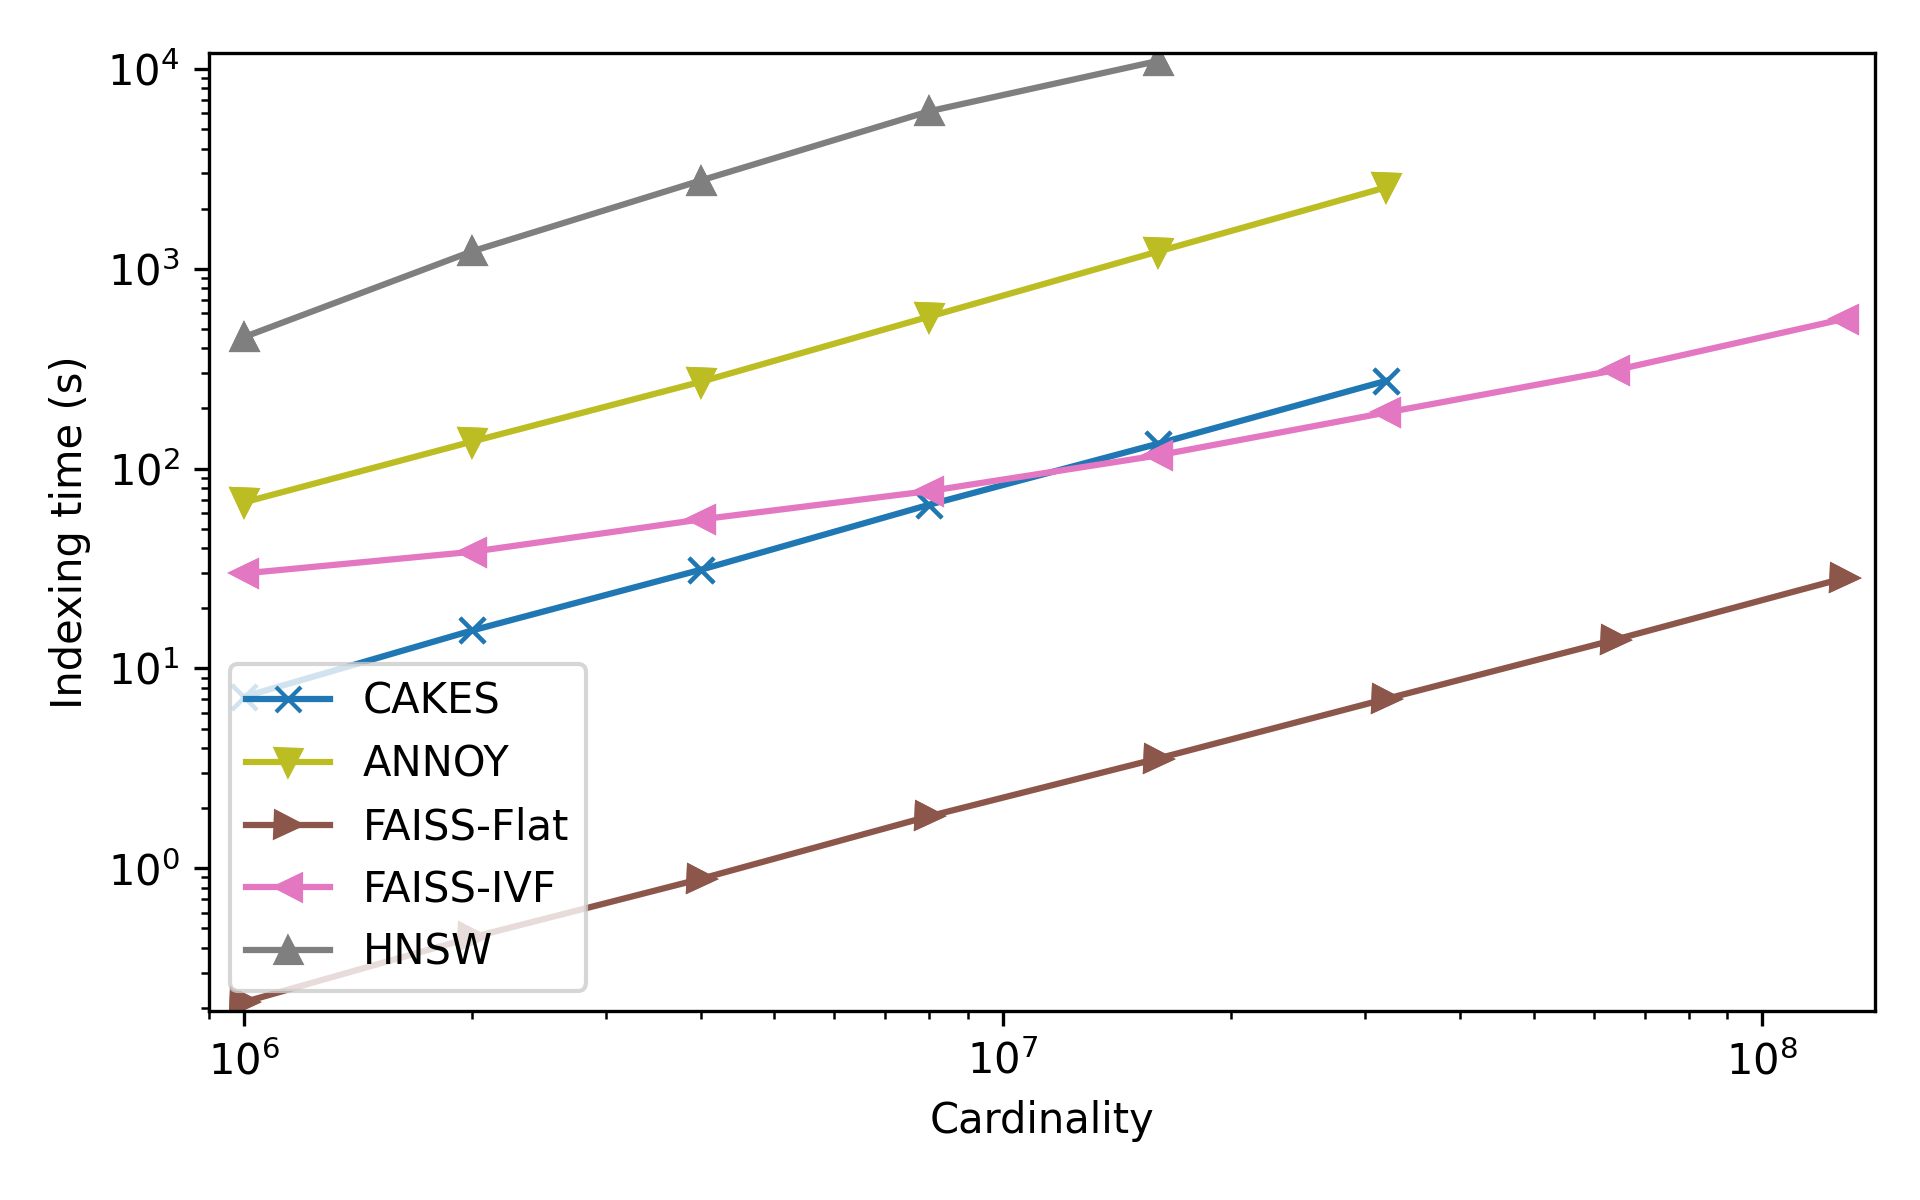
\includegraphics[width=0.95\textwidth]{plots/random-indexing.png}\\
    \subcaption{Random}
    \label{fig:results:random-indexing}
    \end{subfigure}%
    \\
    \vspace{1em}
    \caption{Indexing and tuning time for each algorithm with each of the ANN benchmark datasets and the Random dataset.}
    \label{fig:results:indexing}
\end{figure}


\subsection{Scaling Behavior and Recall}
\label{subsec:scaling-behavior-results}

Figures~\ref{fig:results:fashion-mnist-scaling}, ~\ref{fig:results:glove-25-scaling}, and ~\ref{fig:results:sift-scaling} show the scaling behavior of CAKES algorithms and existing algorithms on augmented versions of the following ann-benchmark datasets: fashion-mnist under Euclidean distance, glove-25 under cosine distance, and sift under Euclidean distance.
Figure~\ref{fig:results:random-scaling} shows the scaling behavior of CAKES algorithms and existing algorithms on a completely randomly generated dataset with same cardinality and dimensionality as sift (1 million points in 128 dimensions).
Figures~\ref{fig:results:silva-scaling} and ~\ref{fig:results:radioml-scaling} show the scaling behavior of CAKES on Silva and RadioML respectively.
The horizontal axis in each figure shows the cardinality of the augmented dataset with synthetic points (see Section \ref{subsec:methods:synthetic-data}).
The left-most point on each line is on the original dataset without any synthetic augmentation.
The vertical axis denotes throughput in queries per second.
Both axes are on a logarithmic scale.
In this section, we report results only for $k$-NN search with $k = 10$, but similar plots for $k=100$ can be found in the Supplement.
For HNSW and ANNOY, we report the recall for each measurement in the plots. For algorithms which exhibit recall greater than $0.9995$, we do not report the recall in the plots, but we do report it in the tables below.


Tables \ref{table:results:ann-fashion}, \ref{table:results:ann-glove-25}, \ref{table:results:ann-sift}, and \ref{table:results:ann-random} show the throughput and recall of CAKES's algorithms at each cardinality for  Fashion-Mnist, Glove-25, Sift, and a random dataset respectively. Though the scaling plots above present results for each of CAKES's three algorithms separately, the results in the CAKES column in these tables represent the fastest CAKES algorithm at that dataset and cardinality only. 
Given that we redo the auto-tuning process described in Section~\ref{subsec:methods:auto-tuning} for each augmented dataset, these values are an accurate representation of CAKES's performance on each dataset and cardinality multiplier. 
When reporting recall, we use 1.000* to denote that the recall is imperfect, but rounds to 1.000 when we consider only three decimal places.

In Figure~\ref{fig:results:fashion-mnist-scaling}, which shows results for Fashion-Mnist, we observe that as cardinality increases, the CAKES algorithms (GreedySieve in blue, Repeated $\rho$-NN in green, and Sieve in purple) are faster than na\"{i}ve linear search (plotted in orange).
In particular, we see that GreedySieve and Sieve begin to exhibit sublinear time performance at a cardinality near $10^5$ (i.e., at a multiplier of about {\color{red} add value} times the original dataset's cardinality). 
We also observe that CAKES's algorithms outperform FAISS-IVF (plotted in pink) for all cardinalities larger than the original dataset's cardinality.
Though state-of-the-art algorithms HNSW (plotted in gray), and ANNOY (plotted in yellow) are faster than CAKES for all cardinalities, we note that CAKES always exhibits perfect recall while HNSW and ANNOY exhibit much lower recall, as shown in Table~\ref{table:results:ann-fashion}.
For example, at a multiplier as low as eight, HNSW and ANNOY have recall of 0.525 and 0.857 respectively,
and this recall gets worse as the multiplier increases.
Meanwhile, CAKES exhibits perfect recall.
Amongst the CAKES algorithms, GreedySieve consistently performs best on this dataset, exhibiting sublinear time performance with increasing multipliers.


With glove-25 (Figure~\ref{fig:results:glove-25-scaling}), we observe that each of CAKES' algorithms outperforms linear search at some cardinality.
Specifically, all three of CAKES' algorithms outperform linear search at a cardinality just slightly more than the original dataset's cardinality, $10^6$.
Similar to the results for Fashion-Mnist, we see that CAKES's algorithms outperform FAISS-IVF for all cardinalities greater than $10^7$.
We see once again that HNSW and ANNOY are faster than CAKES's algorithms for all cardinality multipliers, CAKES's algorithms exhibit better recall at all multipliers, as shown in Table~\ref{table:results:ann-glove-25}.
In particular, at a multiplier as low as two, HNSW and ANNOY have recall as low as 0.607 and 0.832 respectively, and this recall continues to decrease as we increase the multiplier.
In contrast, CAKES exhibits perfect recall at all multipliers.
On this dataset, unlike with fashion-mnist, Repeated $\rho$-NN is consistently the best-performing CAKES algorithm. 


In Figure~\ref{fig:results:sift-scaling}, which displays the scaling behavior of algorithms on the Sift dataset, we observe that while linear search performs best for lower cardinalities, our algorithms begin to outperform our implementation of linear search and FAISS-IVF at a cardinality near $10^7$.
For this dataset, Sieve, is the fastest CAKES algorithm for all cardinalities.
Similar to the results with Fashion-Mnist and Glove-25, we observe that while HNSW and ANNOY are faster than CAKES's algorithms for all cardinality multipliers, CAKES has better recall.
Table~\ref{table:results:ann-sift} shows that even with a multiplier of 1 (i.e., the original dataset), HNSW and ANNOY have recall as low as 0.782 and 0.686 respectively, while CAKES exhibits perfect recall.


With the random dataset, as seen in Figure~\ref{fig:results:random-scaling}, we observe that the three CAKES algorithms are the slowest out of all algorithms, at all cardinalities. 
As with the real datasets, HNSW and ANNOY are the fastest of any of the algorithms, and CAKES exhibits perfect recall at all cardinalities. 
HNSW and ANNOY exhibit \emph{much} lower recall on this random dataset than on the real datasets; 
in particular, with a multiplier of 1, HNSW and ANNOY have recall as low as 0.060 and 0.028 respectively, as reported in Table~\ref{table:results:ann-random}.


For Silva and RadioML, we benchmarked only CAKES's algorithms.
Due to the massive sizes of these datasets, we took random sub-samples of the dataset with lower cardinalities for our benchmarks, rather than augmented versions of the dataset.
With Silva, as shown in Figure~\ref{fig:results:silva-scaling}, we observe that for all algorithms, throughput seems to linearly decrease as cardinality increases, but that it seems to begin levelling off near cardinality $10^5$. Until cardinality near $10^4$, GreedySieve is the fastest CAKES algorithm, but for cardinalities greater than that, Repeated $\rho$-NN is the fastest CAKES algorithm. 
For RadioML, as shown in Figure~\ref{fig:results:radioml-scaling}, we observe that throughput declines nearly linearly the CAKES algorithms exhibit nearly indistinguishable performance for all cardinalities. In particular, throughput of CAKES algorithms is identical within three decimal places for all cardinalities. 

\begin{figure}
\begin{subfigure}[b]{0.47\textwidth}
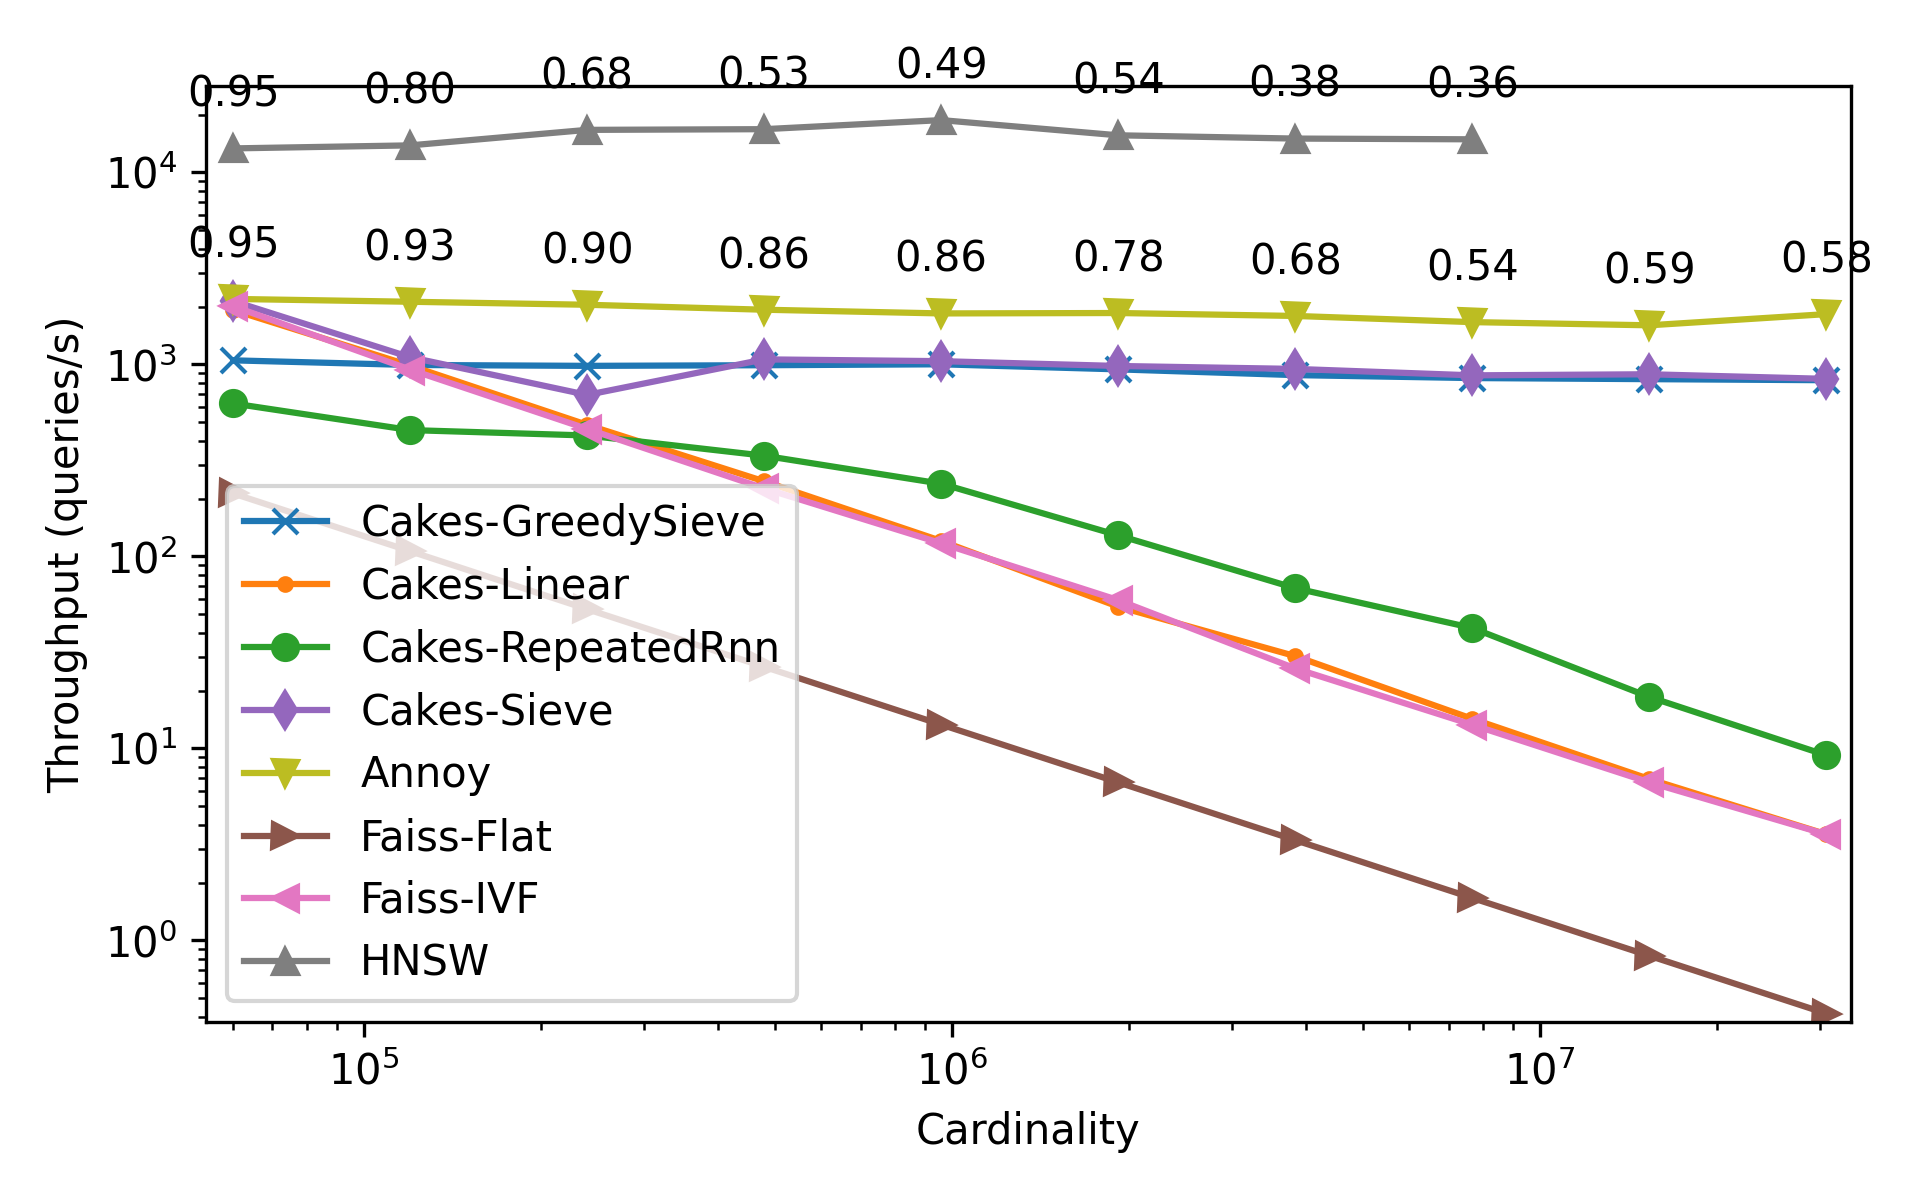
\includegraphics[width=0.95\textwidth]{plots/fashion-mnist-knn-10.png}
\subcaption{Fashion-Mnist for $k=10$.}
\label{fig:results:fashion-mnist-scaling}
\end{subfigure}%
\begin{subfigure}[b]{0.47\textwidth}
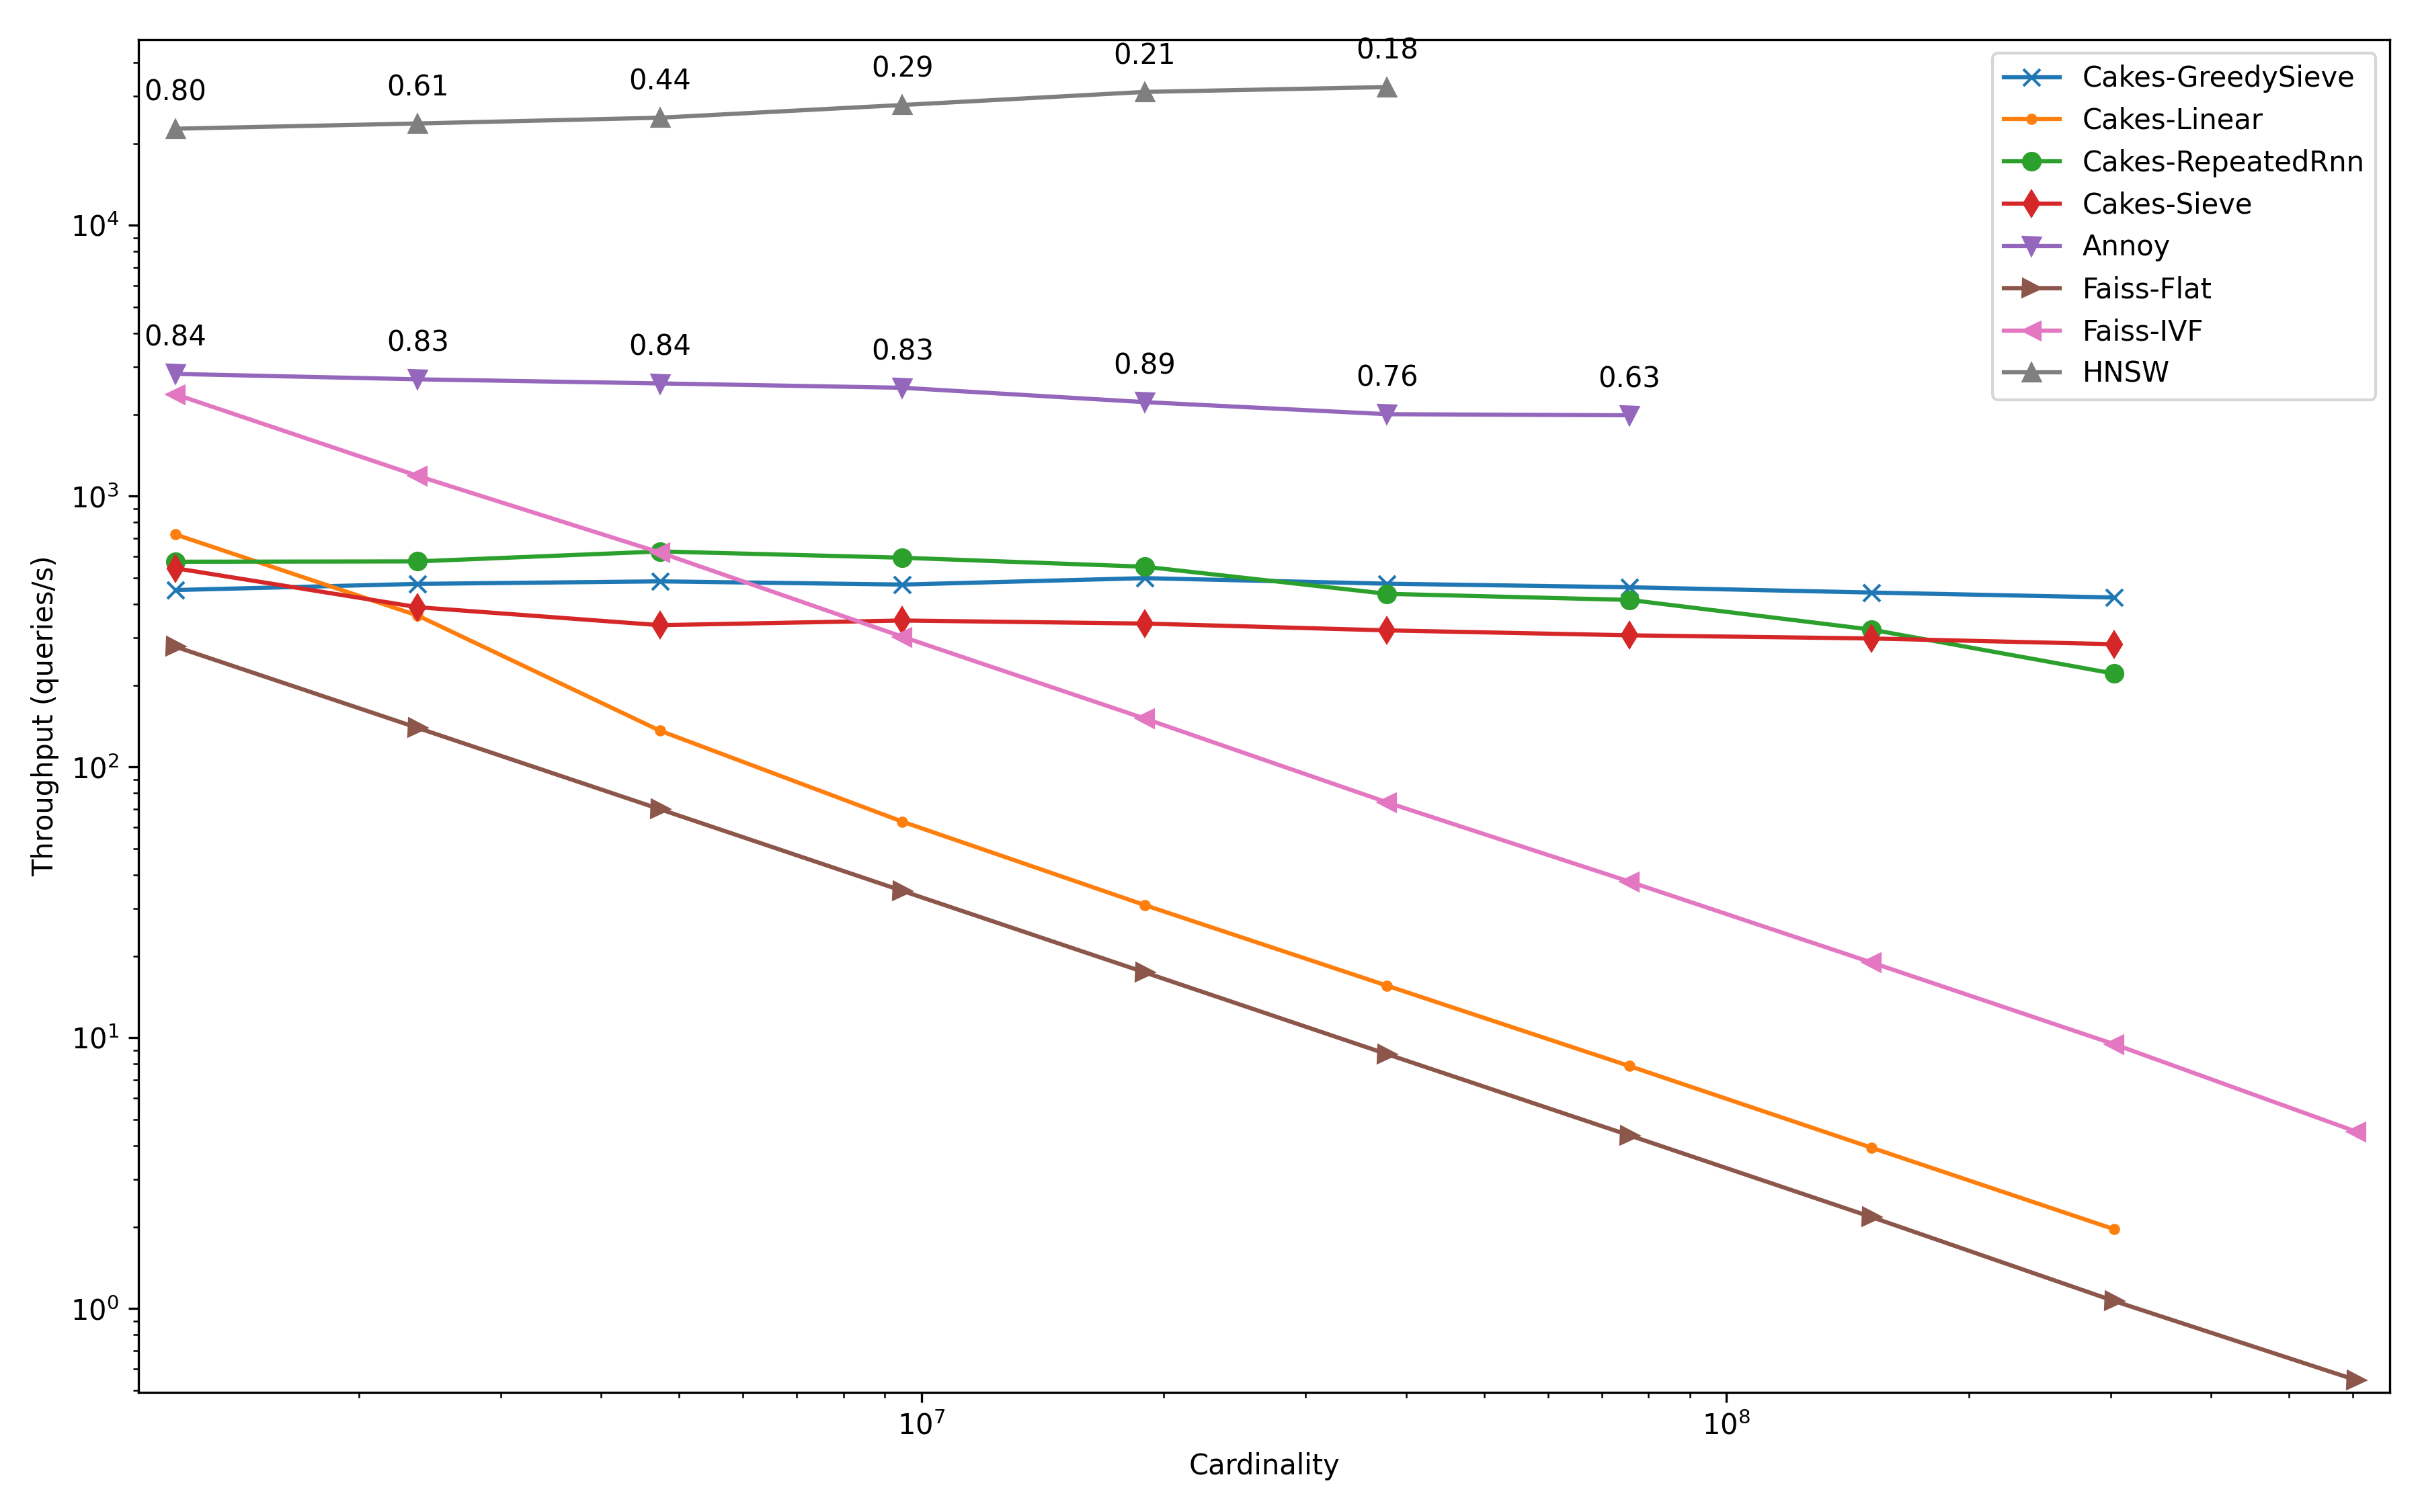
\includegraphics[width=0.95\textwidth]{plots/glove-25-knn-10.png}
\subcaption{Glove-25 for $k=10$.  }
\label{fig:results:glove-25-scaling}
\end{subfigure}%
\vspace{1em}
\\
\begin{subfigure}[b]{0.47\textwidth}
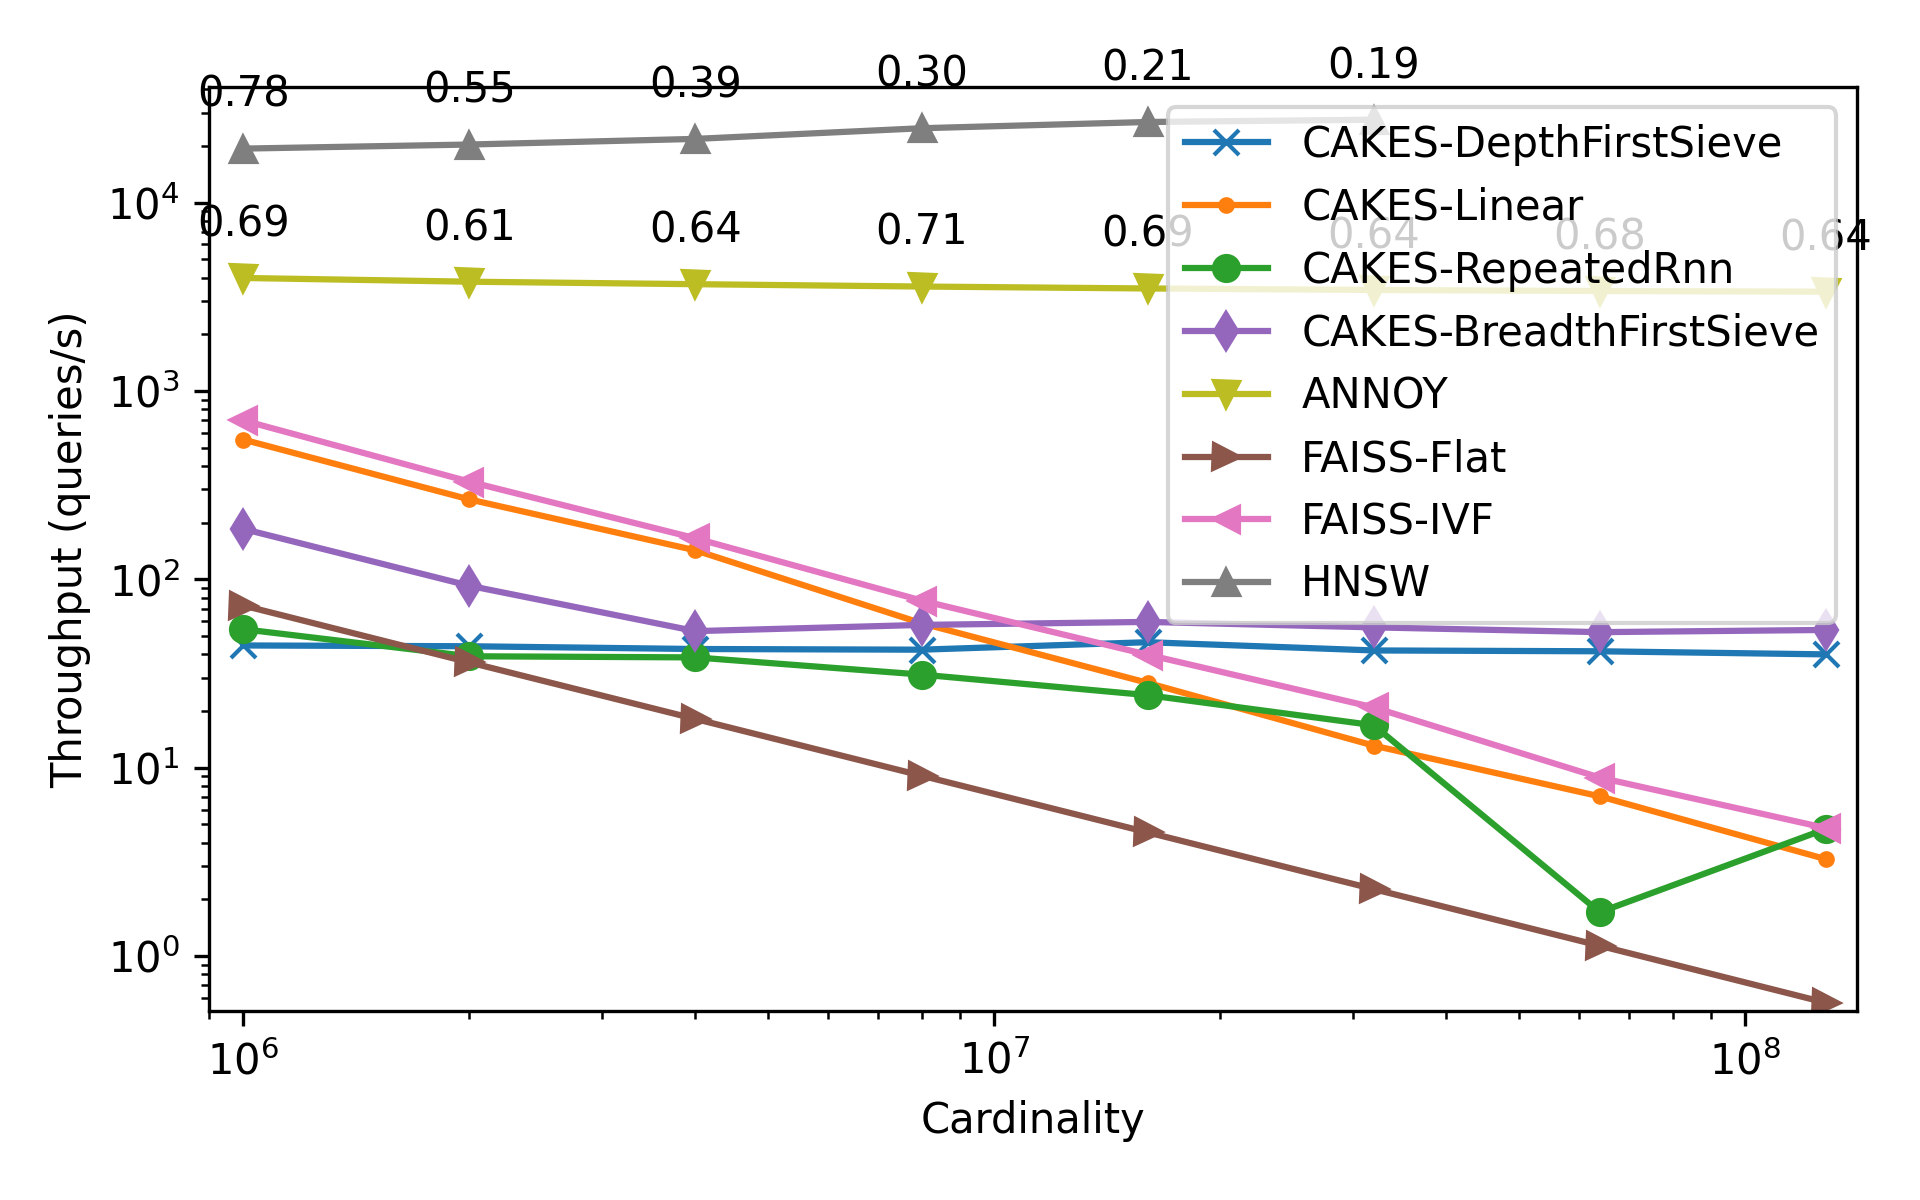
\includegraphics[width=0.95\textwidth]{plots/sift-knn-10.png}
\subcaption{Sift for $k=10$.    }
\label{fig:results:sift-scaling}
\end{subfigure}%
\begin{subfigure}[b]{0.47\textwidth}
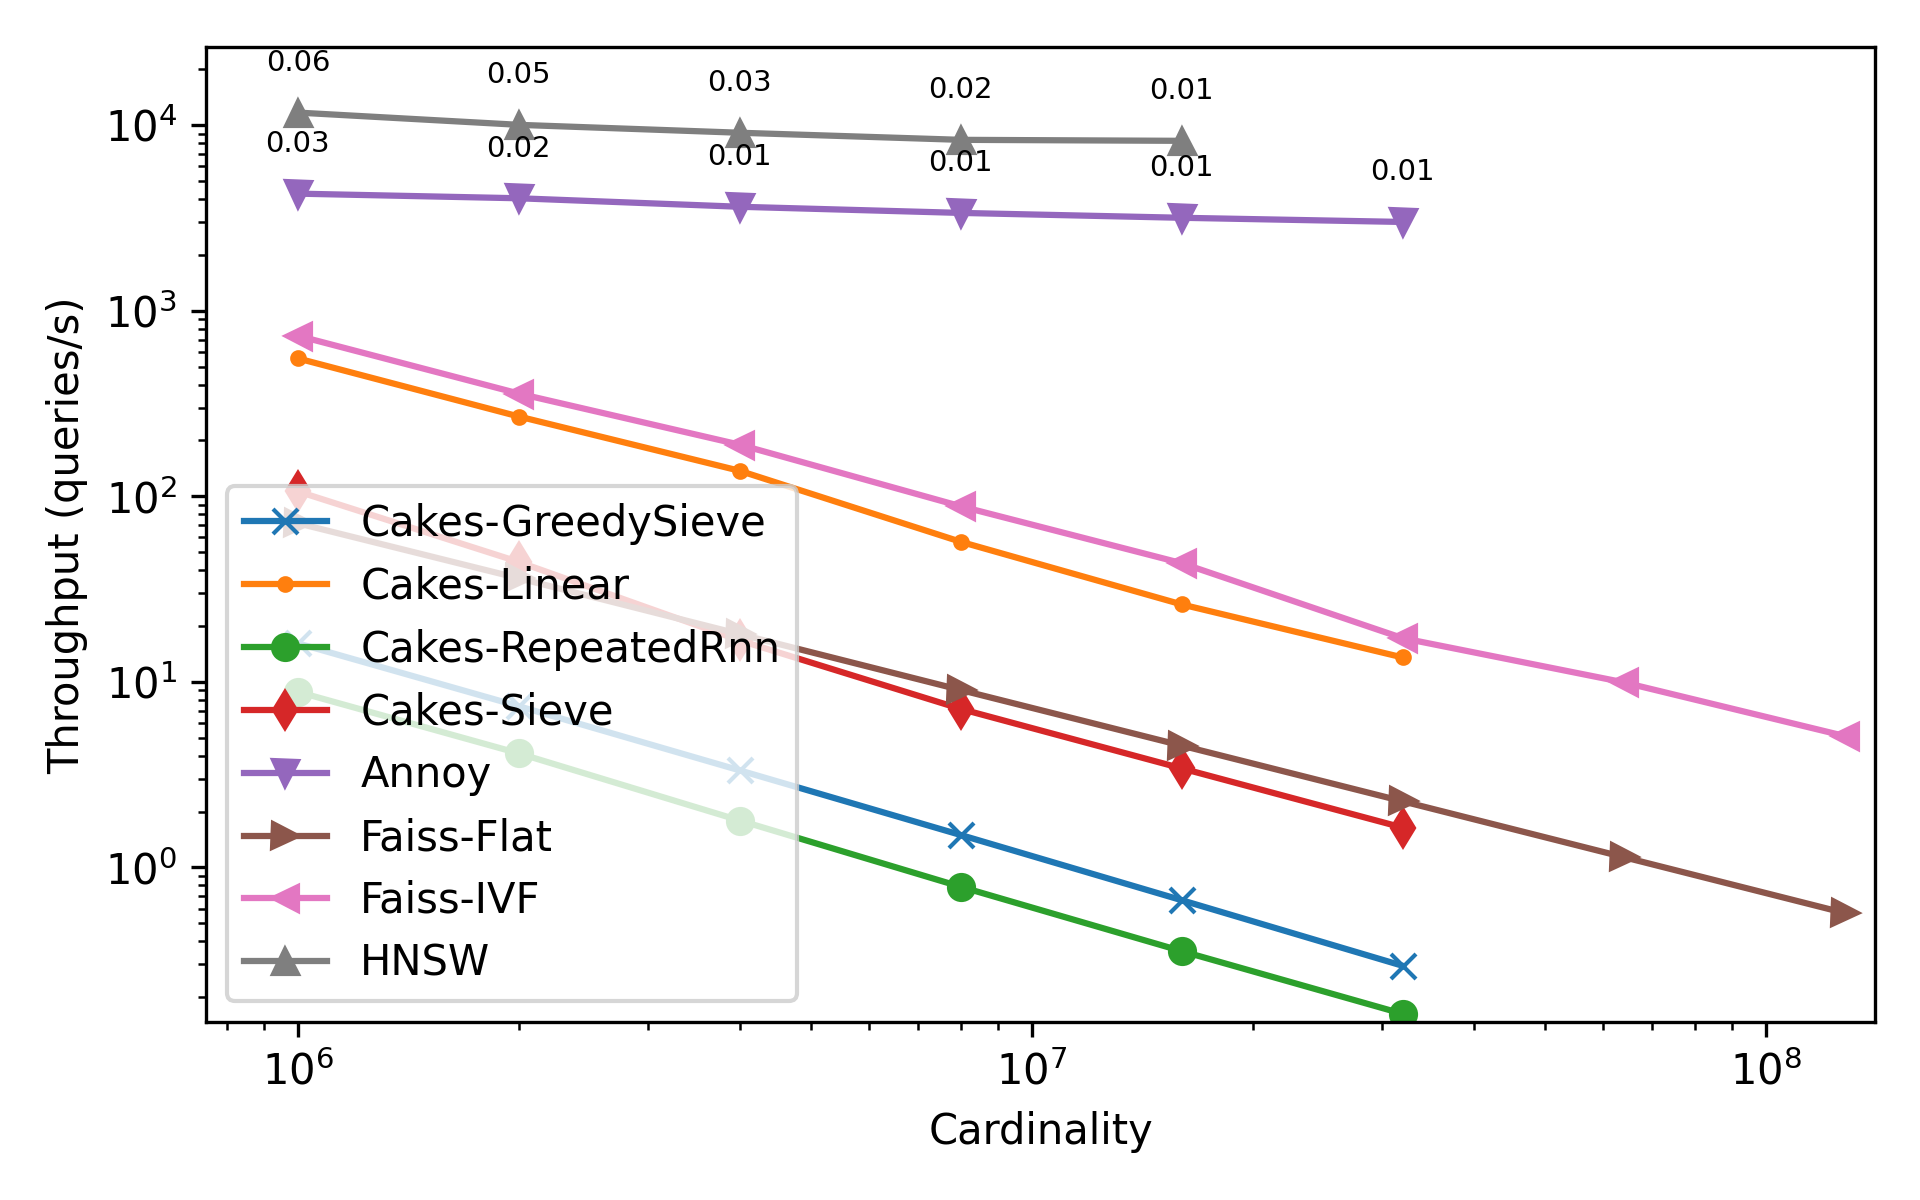
\includegraphics[width=0.95\textwidth]{plots/radio-ml-knn-10.png}
\subcaption{RadioML for $k=10$ at SnR = 10dB.
}
\label{fig:results:radioml-scaling}
\end{subfigure}%
\vspace{1em}
\\
\begin{subfigure}[b]{0.47\textwidth}
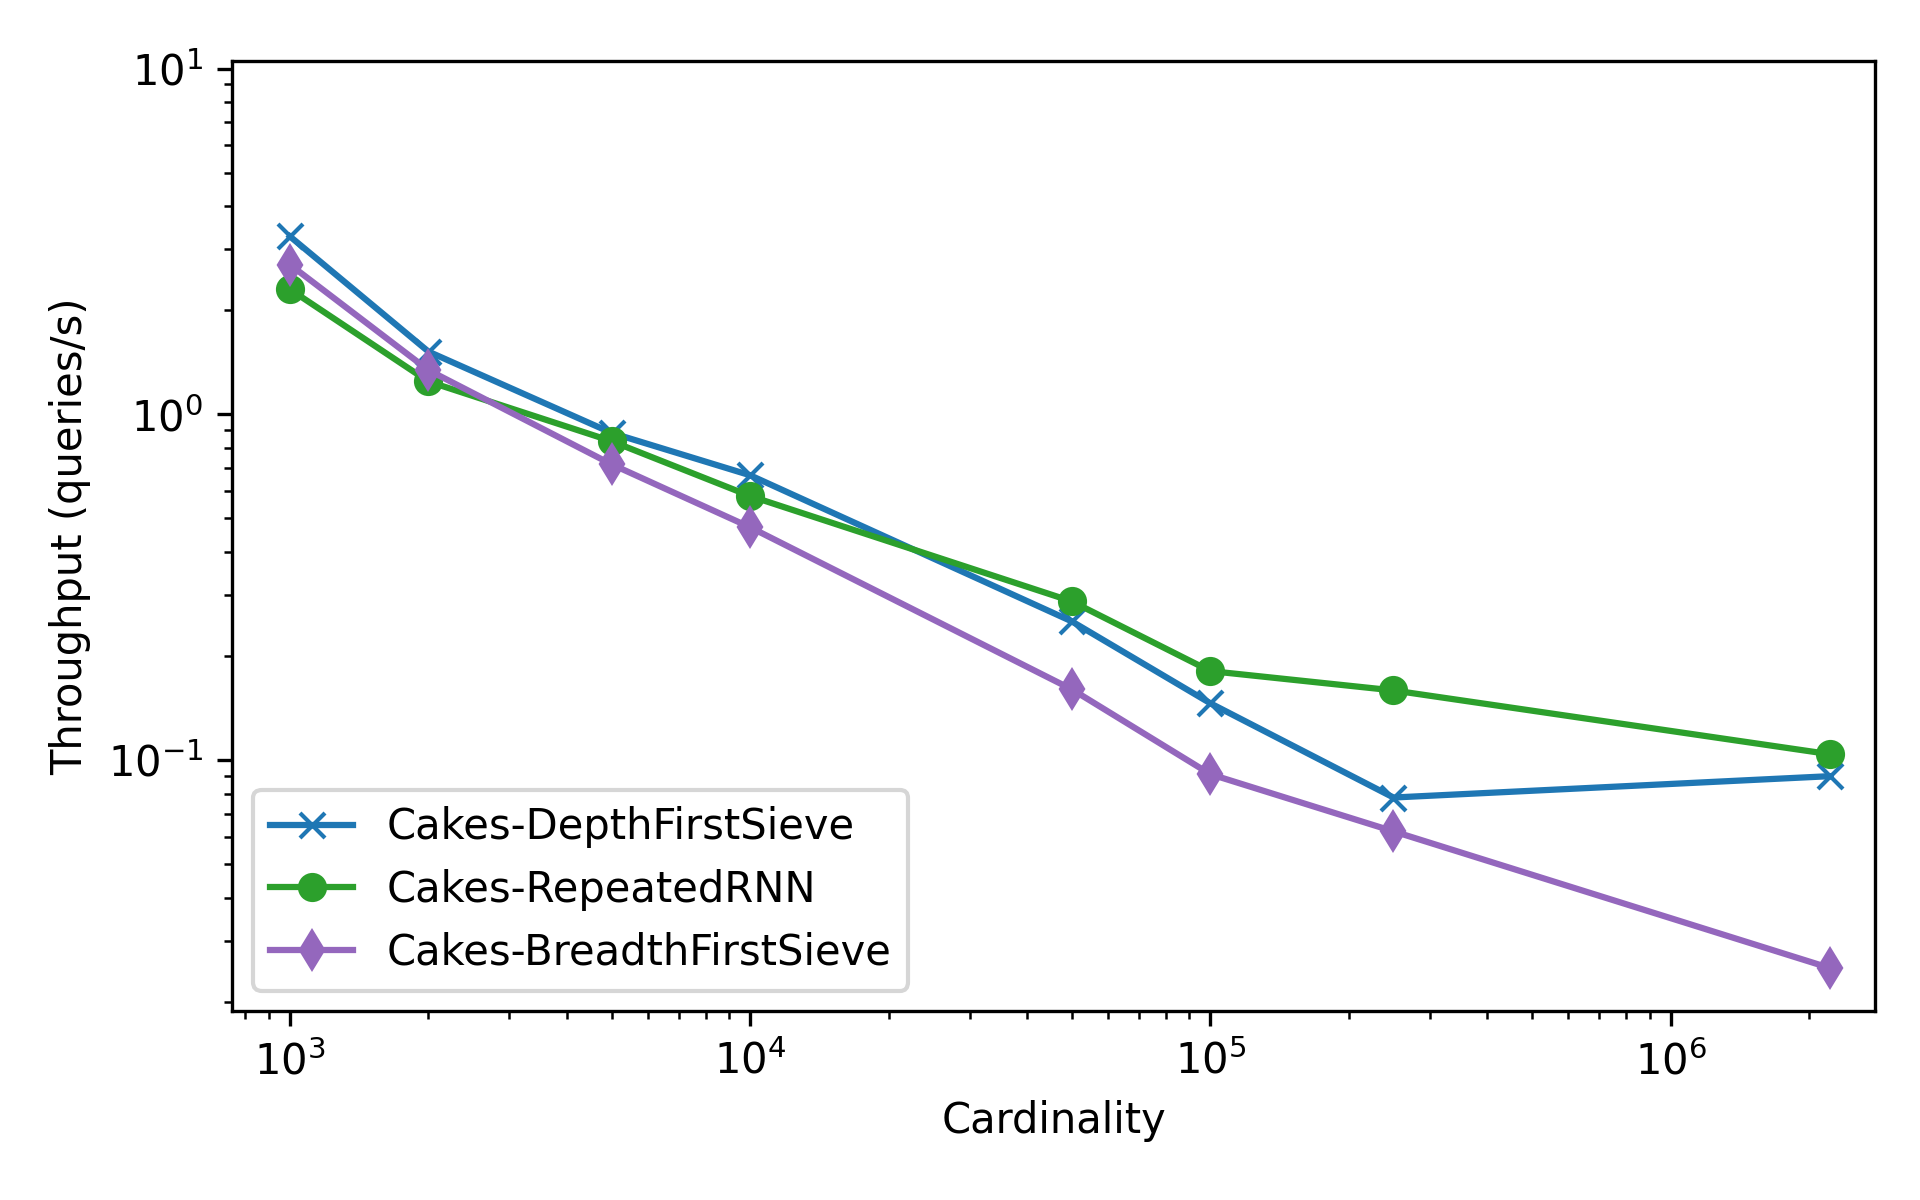
\includegraphics[width=0.95\textwidth]{plots/silva-knn-10.png}
\subcaption{Silva for $k=10$.    }
\label{fig:results:silva-scaling}
\end{subfigure}%
\begin{subfigure}[b]{0.47\textwidth}
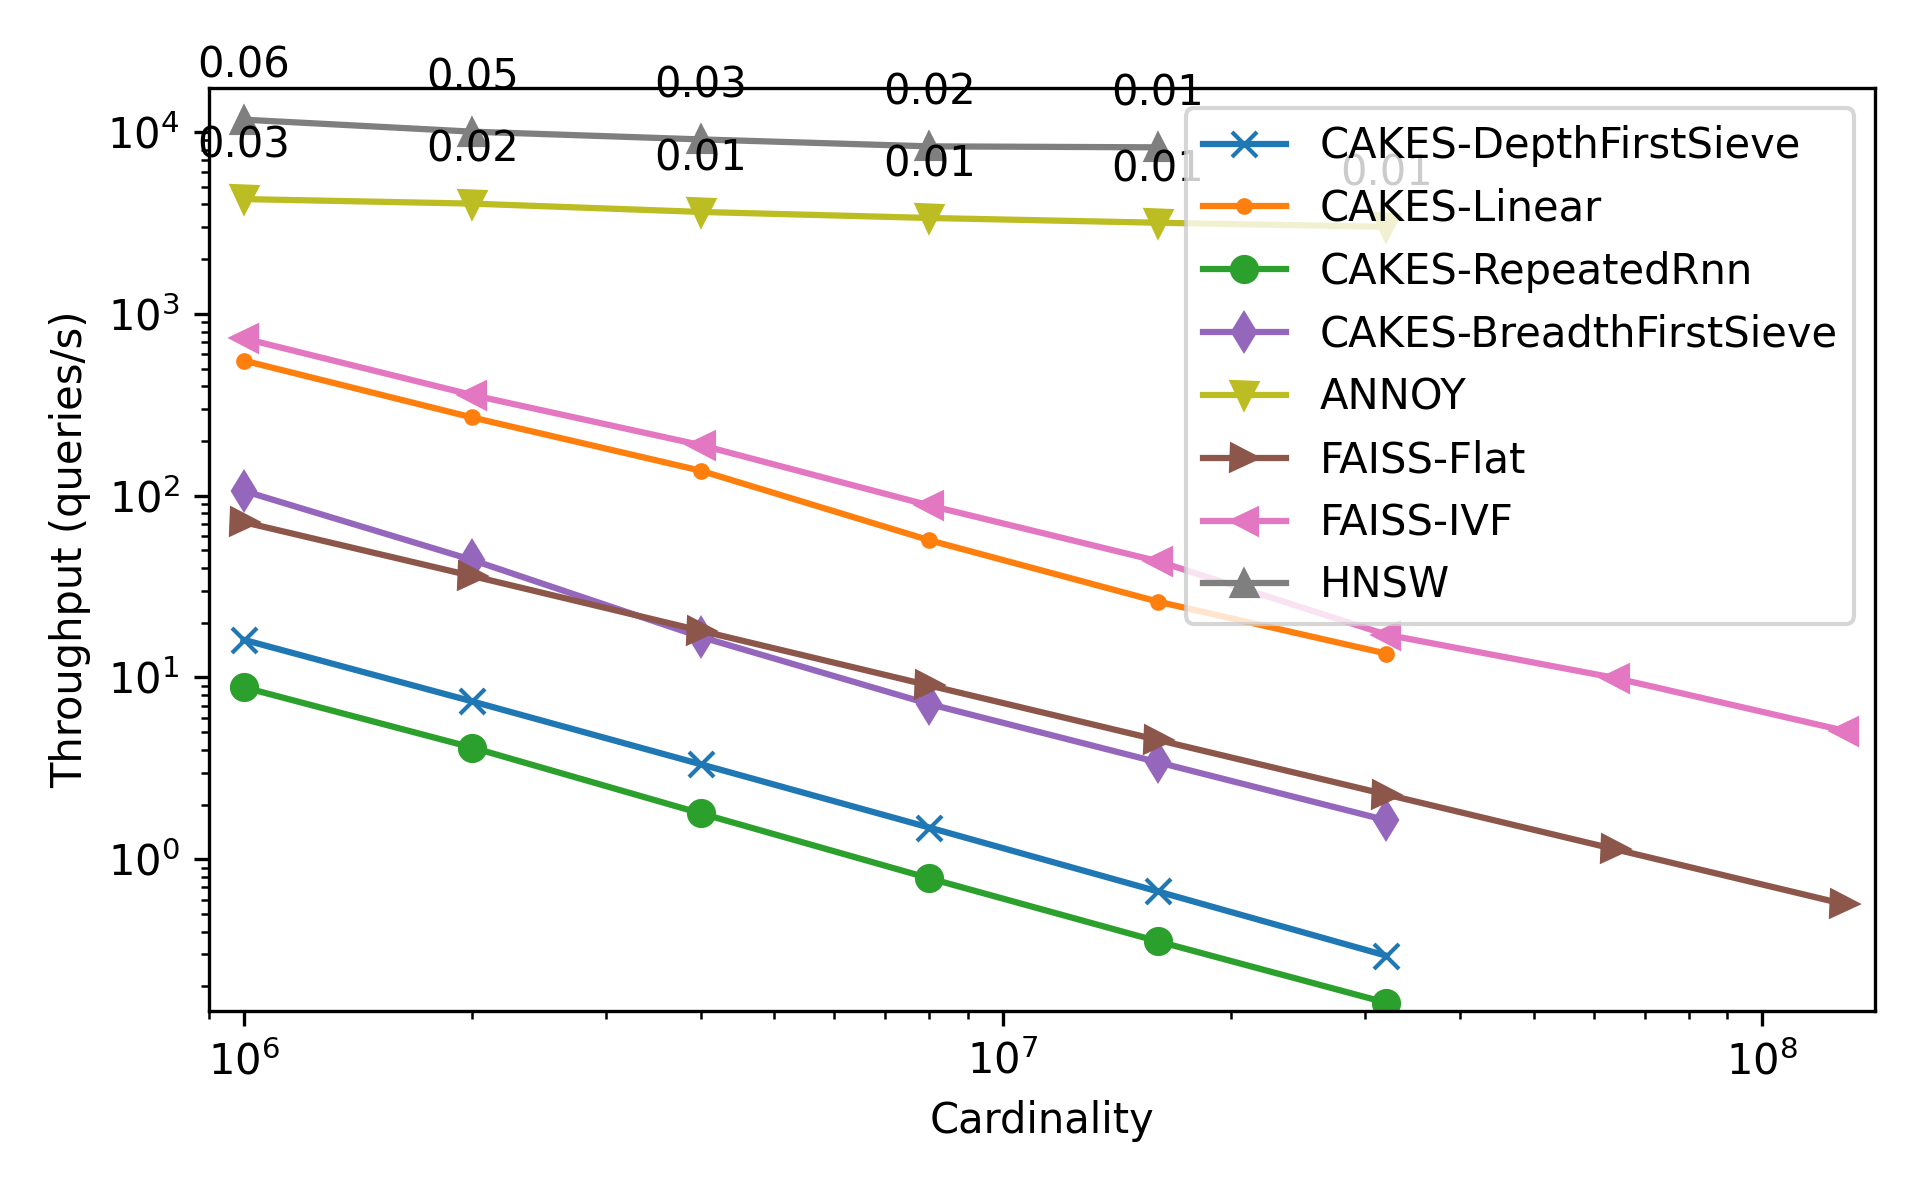
\includegraphics[width=0.95\textwidth]{plots/random-knn-10.png}
\subcaption{A random dataset for $k=10$.
}
\label{fig:results:random-scaling}
\end{subfigure}%


\caption{Algorithm performance across six datasets, including a randomly-generated dataset. In each plot, the horizontal axis represents increasing cardinality (size) of the dataset, while the vertical axis represents the throughput in queries per second (higher is better). For some algorithms, we were not able to take measurements for each cardinality because the index-building took too much memory. {\color{red} Explain this better and be more specific} }
\label{fig:results:scaling-plots}
\end{figure}


\begin{table*}[!t]
    % \renewcommand{\arraystretch}{1.15}
    \caption{Runtime performance (queries per second) and recall on the \textbf{fashion-mnist} dataset. 1.000* denotes imperfect recall that rounds to 1.000.}
    \label{table:results:ann-fashion}
    \vskip 0.15in
    \begin{center}
        \begin{small}
            \begin{sc}
                \begin{tabular}{|l|p{1.2cm}|p{0.8cm}|p{1.2cm}|p{0.8cm}|p{1.2cm}|p{0.8cm}|p{1.2cm}|p{0.8cm}|p{1.2cm}|p{0.8cm}|}
                    \hline
                    \textbf{Multiplier}  & \multicolumn{2}{|c|}{\textbf{hnsw}} & \multicolumn{2}{|c|}{\textbf{annoy}} & \multicolumn{2}{|c|}{\textbf{faiss-flat}} & \multicolumn{2}{|c|}{\textbf{faiss-ivf}}  & \multicolumn{2}{|c|}{\textbf{CAKES}} \\
                    \hline
                    &             QPS & Recall        & QPS & Recall      & QPS & Recall       & QPS & Recall     & QPS & Recall    \\
                    \hline
                    1   & 1.33~$\times10^{4}$ & 0.954 & 2.19~$\times10^{3}$ & 0.950 & 2.13~$\times10^{2}$  & 1.000 & 2.01~$\times10^{3}$ & 1.000* & 2.17~$\times10^{3}$ & 1.000 \\
                    \hline
                    2   & 1.38~$\times10^{4}$ & 0.803 & 2.12~$\times10^{3}$ & 0.927 & 1.06~$\times10^{2}$  & 1.000 & 9.39~$\times10^{2}$ & 1.000* & 1.14~$\times10^{3}$ & 1.000 \\
                    \hline
                    4   & 1.66~$\times10^{4}$ & 0.681 & 2.04~$\times10^{3}$ & 0.898 & 5.31~$\times10^{1}$  & 1.000 & 4.61~$\times10^{2}$ & 0.997  & 9.82~$\times10^{2}$ & 1.000 \\
                    \hline
                    8   & 1.68~$\times10^{4}$ & 0.525 & 1.93~$\times10^{3}$ & 0.857 & 2.66~$\times10^{1}$  & 1.000 & 2.26~$\times10^{2}$ & 0.995  & 1.18~$\times10^{3}$ & 1.000 \\
                    \hline
                    16  & 1.87~$\times10^{4}$ & 0.494 & 1.84~$\times10^{3}$ & 0.862 & 1.33~$\times10^{1}$  & 1.000 & 1.17~$\times10^{2}$ & 0.991  & 1.20~$\times10^{3}$ & 1.000 \\
                    \hline
                    32  & 1.56~$\times10^{4}$ & 0.542 & 1.85~$\times10^{3}$ & 0.775 & 6.65~$\times10^{0}$  & 1.000 & 5.91~$\times10^{1}$ & 0.985  & 1.16~$\times10^{3}$ & 1.000 \\
                    \hline
                    64  & 1.50~$\times10^{4}$ & 0.378 & 1.78~$\times10^{3}$ & 0.677 & 3.32~$\times10^{0}$  & 1.000 & 2.61~$\times10^{1}$ & 0.968  & 1.10~$\times10^{3}$ & 1.000 \\
                    \hline
                    128 & 1.49~$\times10^{4}$ & 0.357 & 1.66~$\times10^{3}$ & 0.538 & 1.66~$\times10^{0}$  & 1.000 & 1.33~$\times10^{1}$ & 0.964  & 1.04~$\times10^{3}$ & 1.000 \\
                    \hline
                    256 & --                  & --    & 1.60~$\times10^{3}$ & 0.592 & 8.31~$\times10^{-1}$ & 1.000 & 6.65~$\times10^{0}$ & 0.962  & 1.06~$\times10^{3}$ & 1.000 \\
                    \hline
                    512 & --                  & --    & 1.83~$\times10^{3}$ & 0.581 & 4.16~$\times10^{-1}$ & 1.000 & 3.56~$\times10^{0}$ & 0.949  & 1.04~$\times10^{3}$ & 1.000 \\
                    \hline
                \end{tabular}
            \end{sc}
        \end{small}
    \end{center}
    \vskip -0.1in
\end{table*}


\begin{table*}[!t]
    % \renewcommand{\arraystretch}{1.15}
    \caption{Runtime performance (queries per second) and recall on the \textbf{glove-25} dataset. 1.000* denotes imperfect recall that rounds to 1.000.}
    \label{table:results:ann-glove-25}
    \vskip 0.15in
    \begin{center}
        \begin{small}
            \begin{sc}
                \begin{tabular}{|l|p{1.2cm}|p{0.8cm}|p{1.2cm}|p{0.8cm}|p{1.2cm}|p{0.8cm}|p{1.2cm}|p{0.8cm}|p{1.2cm}|p{0.8cm}|}
                    \hline
                    \textbf{Multiplier}  & \multicolumn{2}{|c|}{\textbf{hnsw}} & \multicolumn{2}{|c|}{\textbf{annoy}} & \multicolumn{2}{|c|}{\textbf{faiss-flat}} & \multicolumn{2}{|c|}{\textbf{faiss-ivf}}  & \multicolumn{2}{|c|}{\textbf{CAKES}} \\
                    \hline
                    &             QPS & Recall        & QPS & Recall      & QPS & Recall       & QPS & Recall     & QPS & Recall    \\
                    \hline
                    1   & 2.28~$\times10^{4}$ & 0.801 & 2.83~$\times10^{3}$ & 0.835 & 2.78~$\times10^{2}$ & 1.000 & 2.38~$\times10^{3}$ & 1.000* & 7.22~$\times10^{2}$ & 1.000* \\
                    \hline
                    2   & 2.38~$\times10^{4}$ & 0.607 & 2.70~$\times10^{3}$ & 0.832 & 1.39~$\times10^{2}$ & 1.000 & 1.19~$\times10^{3}$ & 1.000* & 5.75~$\times10^{2}$ & 1.000* \\
                    \hline
                    4   & 2.50~$\times10^{4}$ & 0.443 & 2.61~$\times10^{3}$ & 0.839 & 6.98~$\times10^{1}$ & 1.000 & 6.19~$\times10^{2}$ & 1.000* & 6.25~$\times10^{2}$ & 1.000* \\
                    \hline
                    8   & 2.78~$\times10^{4}$ & 0.294 & 2.51~$\times10^{3}$ & 0.834 & 3.49~$\times10^{1}$ & 1.000 & 3.03~$\times10^{2}$ & 1.000* & 5.93~$\times10^{2}$ & 1.000* \\
                    \hline
                    16  & 3.11~$\times10^{4}$ & 0.213 & 2.23~$\times10^{3}$ & 0.885 & 1.74~$\times10^{1}$ & 1.000 & 1.51~$\times10^{2}$ & 1.000* & 5.49~$\times10^{2}$ & 1.000* \\
                    \hline
                    32  & 3.24~$\times10^{4}$ & 0.178 & 2.01~$\times10^{3}$ & 0.764 & 8.70~$\times10^{0}$ & 1.000 & 7.40~$\times10^{1}$ & 0.999  & 4.75~$\times10^{2}$ & 1.000* \\
                    \hline
                    64  & --                  & --    & 1.99~$\times10^{3}$ & 0.631 & 4.36~$\times10^{0}$ & 1.000 & 3.77~$\times10^{1}$ & 0.997  & 4.61~$\times10^{2}$ & 1.000* \\
                    \hline
                    128 & --                  & --    & --                  & --    & 2.18~$\times10^{0}$ & 1.000 & 1.90~$\times10^{1}$ & 0.998  & 4.41~$\times10^{2}$ & 1.000* \\
                    \hline
                    256 & --                  & --    & --                  & --    & 1.07~$\times10^{0}$ & 1.000 & 9.47~$\times10^{0}$ & 0.998  & 4.23~$\times10^{2}$ & 1.000* \\
                    \hline
                    % 512 & -- & -- & -- & -- & 0.544 & 1.000 & 4.499 & 0.996 & 0.000 & 0.000 \\
                    % \hline
                \end{tabular}
            \end{sc}
        \end{small}
    \end{center}
    \vskip -0.1in
\end{table*}

\begin{table*}[!t]
    % \renewcommand{\arraystretch}{1.15}
    \caption{Runtime performance (queries per second) and recall on the \textbf{sift} dataset. 1.000* denotes imperfect recall that rounds to 1.000.}
    \label{table:results:ann-sift}
    \vskip 0.15in
    \begin{center}
        \begin{small}
            \begin{sc}
                \begin{tabular}{|l|p{1.2cm}|p{0.8cm}|p{1.2cm}|p{0.8cm}|p{1.2cm}|p{0.8cm}|p{1.2cm}|p{0.8cm}|p{1.2cm}|p{0.8cm}|}
                    \hline
                    \textbf{Multiplier}  & \multicolumn{2}{|c|}{\textbf{hnsw}}  & \multicolumn{2}{|c|}{\textbf{annoy}} & \multicolumn{2}{|c|}{\textbf{faiss-flat}} & \multicolumn{2}{|c|}{\textbf{faiss-ivf-flat}}  & \multicolumn{2}{|c|}{\textbf{CAKES}} \\
                    \hline
                    &             QPS & Recall        & QPS & Recall      & QPS & Recall       & QPS & Recall    & QPS & Recall    \\
                    \hline
                    1   & 1.93~$\times10^{4}$ & 0.782 & 3.98~$\times10^{3}$ & 0.686 & 7.26~$\times10^{1}$  & 1.000 & 6.98~$\times10^{2}$ & 1.000* & 5.52~$\times10^{2}$ & 1.000 \\
                    \hline
                    2   & 2.03~$\times10^{4}$ & 0.552 & 3.80~$\times10^{3}$ & 0.614 & 3.62~$\times10^{1}$  & 1.000 & 3.30~$\times10^{2}$ & 1.000* & 2.66~$\times10^{2}$ & 1.000 \\
                    \hline
                    4   & 2.18~$\times10^{4}$ & 0.394 & 3.69~$\times10^{3}$ & 0.637 & 1.82~$\times10^{1}$  & 1.000 & 1.65~$\times10^{2}$ & 1.000* & 1.43~$\times10^{2}$ & 1.000 \\
                    \hline
                    8   & 2.48~$\times10^{4}$ & 0.298 & 3.58~$\times10^{3}$ & 0.710 & 9.08~$\times10^{0}$  & 1.000 & 7.72~$\times10^{1}$ & 1.000* & 7.94~$\times10^{1}$ & 1.000 \\
                    \hline
                    16  & 2.68~$\times10^{4}$ & 0.210 & 3.50~$\times10^{3}$ & 0.690 & 4.54~$\times10^{0}$  & 1.000 & 3.98~$\times10^{1}$ & 1.000* & 8.12~$\times10^{1}$ & 1.000 \\
                    \hline
                    32  & 2.75~$\times10^{4}$ & 0.193 & 3.44~$\times10^{3}$ & 0.639 & 2.27~$\times10^{0}$  & 1.000 & 2.09~$\times10^{1}$ & 0.999  & 7.81~$\times10^{1}$ & 1.000 \\
                    \hline
                    64  & --                  & --    & 3.39~$\times10^{3}$ & 0.678 & 1.14~$\times10^{0}$  & 1.000 & 8.87~$\times10^{0}$ & 0.997  & 7.43~$\times10^{1}$ & 1.000 \\
                    \hline
                    128 & --                  & --    & 3.36~$\times10^{3}$ & 0.643 & 5.66~$\times10^{-1}$ & 1.000 & 4.78~$\times10^{0}$ & 0.993  & 6.80~$\times10^{1}$ & 1.000 \\
                    \hline
                \end{tabular}
            \end{sc}
        \end{small}
    \end{center}
    \vskip -0.1in
\end{table*}


\begin{table*}[!t]
    % \renewcommand{\arraystretch}{1.15}
    \caption{Runtime performance (queries per second) and recall on a \textbf{random} dataset. 1.000* denotes imperfect recall that rounds to 1.000.}
    \label{table:results:ann-random}
    \vskip 0.15in
    \begin{center}
        \begin{small}
            \begin{sc}
                \begin{tabular}{|l|p{1.2cm}|p{0.8cm}|p{1.2cm}|p{0.8cm}|p{1.2cm}|p{0.8cm}|p{1.2cm}|p{0.8cm}|p{1.2cm}|p{0.8cm}|}
                    \hline
                    \textbf{Multiplier}  & \multicolumn{2}{|c|}{\textbf{hnsw}}  & \multicolumn{2}{|c|}{\textbf{annoy}} & \multicolumn{2}{|c|}{\textbf{faiss-flat}} & \multicolumn{2}{|c|}{\textbf{faiss-ivf-flat}}  & \multicolumn{2}{|c|}{\textbf{CAKES}} \\
                    \hline
                    &             QPS & Recall        & QPS & Recall      & QPS & Recall       & QPS & Recall    & QPS & Recall    \\
                    \hline
                    1  & 1.17~$\times10^{4}$ & 0.060 & 4.28~$\times10^{3}$ & 0.028 & 7.16~$\times10^{1}$ & 1.000 & 7.34~$\times10^{2}$ & 1.000* & 5.54~$\times10^{2}$ & 1.000 \\
                    \hline
                    2  & 1.01~$\times10^{4}$ & 0.048 & 4.04~$\times10^{3}$ & 0.021 & 3.62~$\times10^{1}$ & 1.000 & 3.58~$\times10^{2}$ & 1.000* & 2.69~$\times10^{2}$ & 1.000 \\
                    \hline
                    4  & 9.12~$\times10^{3}$ & 0.031 & 3.64~$\times10^{3}$ & 0.014 & 1.81~$\times10^{1}$ & 1.000 & 1.90~$\times10^{2}$ & 1.000* & 1.37~$\times10^{2}$ & 1.000 \\
                    \hline
                    8  & 8.35~$\times10^{3}$ & 0.022 & 3.37~$\times10^{3}$ & 0.013 & 9.04~$\times10^{0}$ & 1.000 & 8.84~$\times10^{1}$ & 1.000* & 5.69~$\times10^{1}$ & 1.000 \\
                    \hline
                    16 & 8.25~$\times10^{3}$ & 0.008 & 3.17~$\times10^{3}$ & 0.006 & 4.53~$\times10^{0}$ & 1.000 & 4.36~$\times10^{1}$ & 1.000* & 2.61~$\times10^{1}$ & 1.000 \\
                    \hline
                    32 & --                  & --    & 3.01~$\times10^{3}$ & 0.007 & 2.27~$\times10^{0}$ & 1.000 & 1.72~$\times10^{1}$ & 1.000* & 1.35~$\times10^{1}$ & 1.000 \\
                    % \hline
                    % 64 & -- & -- & -- & -- & 1.135 & 1.000 & 9.939 & 1.000 & 0.000 & 0.000 \\
                    % \hline
                    % 128 & --& -- & -- & -- & 0.567 & 1.000 & 5.106 & 1.000 & 0.000 & 0.000 \\
                    \hline
                \end{tabular}
            \end{sc}
        \end{small}
    \end{center}
    \vskip -0.1in
\end{table*}

